\documentclass[UTF8,fontset=fandol,zihao=-4,a4paper]{ctexart}

\usepackage[top=2.25cm,bottom=2.20cm,left=2.35cm,right=2.35cm]{geometry}
\usepackage{fontspec}
\usepackage{amsmath,amssymb,bm,mathtools}
\usepackage{booktabs,longtable,tabularx,array,multirow,makecell}
\usepackage{graphicx,adjustbox,caption,subcaption,float}
\usepackage[section]{placeins}
\usepackage{flafter}
\usepackage{tikz}
\usetikzlibrary{arrows.meta,calc,positioning,shapes.geometric,decorations.pathreplacing,fit,backgrounds}
\usepackage{siunitx}
\usepackage{enumitem}
\usepackage{fancyhdr}
\usepackage{xcolor}
\usepackage{hyperref}
\usepackage{bookmark}
\usepackage{url}
\usepackage{threeparttable}
\usepackage{microtype}

\graphicspath{{figures/}{standalone_reference_reproductions/}}
\definecolor{papergray}{gray}{0.32}
\definecolor{MaleBlue}{HTML}{2D75A8}
\definecolor{FemaleRed}{HTML}{C9564B}
\definecolor{Slate}{HTML}{66788A}
\definecolor{Gold}{HTML}{D79A25}
\hypersetup{
  hidelinks,
  pdfauthor={},
  pdftitle={可靠性约束下的NIPT检测时点优化与染色体异常判定}
}
\captionsetup{font=small,labelsep=quad,skip=6pt,justification=centering,singlelinecheck=true}
\captionsetup[table]{position=top,skip=5pt}
\sisetup{detect-all,group-separator={,},group-minimum-digits=5}
\setlist{nosep,leftmargin=2em}
\setlength{\parindent}{2em}
\setlength{\parskip}{0pt}
\linespread{1.30}
\setlength{\emergencystretch}{2em}
\setlength{\abovedisplayskip}{7pt plus 2pt minus 2pt}
\setlength{\belowdisplayskip}{7pt plus 2pt minus 2pt}
\setlength{\textfloatsep}{10pt plus 2pt minus 2pt}
\setlength{\floatsep}{8pt plus 2pt minus 2pt}
\setlength{\intextsep}{8pt plus 2pt minus 2pt}
\renewcommand{\topfraction}{0.92}
\renewcommand{\bottomfraction}{0.88}
\renewcommand{\textfraction}{0.06}
\renewcommand{\floatpagefraction}{0.78}
\setcounter{topnumber}{3}
\setcounter{bottomnumber}{2}
\setcounter{totalnumber}{5}
\renewcommand{\arraystretch}{1.18}
\setlength{\tabcolsep}{4pt}
\setlength{\LTleft}{0pt}
\setlength{\LTright}{0pt}

\newcolumntype{L}{>{\raggedright\arraybackslash}X}
\newcolumntype{C}{>{\centering\arraybackslash}X}
\newcolumntype{R}{>{\raggedleft\arraybackslash}X}
\newcolumntype{P}[1]{>{\raggedright\arraybackslash}p{#1}}
\newcolumntype{Q}[1]{>{\centering\arraybackslash}p{#1}}
\newcommand{\dif}{\mathop{}\!\mathrm{d}}
\newcommand{\R}{\mathbb{R}}
\newcommand{\vect}[1]{\bm{#1}}
\newcommand{\pandocbounded}[1]{#1}
\providecommand{\tightlist}{\setlength{\itemsep}{0pt}\setlength{\parskip}{0pt}}
\providecommand{\passthrough}[1]{#1}

\setcounter{secnumdepth}{0}
\ctexset{
  section={format=\centering\heiti\zihao{3},beforeskip=12pt,afterskip=8pt},
  subsection={format=\heiti\zihao{4},beforeskip=9pt,afterskip=5pt},
  subsubsection={format=\heiti\zihao{-4},beforeskip=7pt,afterskip=3pt}
}

\pagestyle{fancy}
\fancyhf{}
\fancyhead[C]{\zihao{-5}可靠性约束下的 NIPT 检测时点优化与染色体异常判定}
\fancyfoot[C]{\thepage}
\renewcommand{\headrulewidth}{0.4pt}
\setlength{\headheight}{14pt}

\begin{document}
\pagenumbering{gobble}
\begin{center}
  {\heiti\zihao{2}可靠性约束下的 NIPT 检测时点优化\par}
  \vspace{0.35em}
  {\heiti\zihao{3}——男胎检测时点与女胎染色体异常的统一建模\par}
  \vspace{1.0em}
\end{center}

\noindent{\heiti 摘要：}

在临床实践中，NIPT 通过采集母体外周血检测胎儿游离 DNA
片段，其准确性受检测时点与孕妇个体特征匹配程度的影响。Y
染色体浓度随孕周动态变化，技术测量误差贯穿检测全流程，异常标签在女胎数据中尤为稀疏，这些因素共同使决策面临多重不确定性。本文将男胎检测时点选择转化为可靠性约束下的分组排程问题，将女胎异常判定转化为孕妇等权的多标签稀疏筛查问题，围绕同一套数据层级结构，依次建立了浓度关系模型、达标时间分布模型、分组优化模型与异常概率模型。

针对问题一，本文采用对数几率变换处理有界浓度。在采血事件层聚合技术复测后，建立
18 周分段线性随机截距混合模型，并将 BMI
分解为基线值与孕期内变化量。组内相关系数为 0.7304，73.0\%
的浓度变异来自孕妇间稳定差异。18 周前孕周斜率为 0.02338，其后总斜率增至
0.06315，基线 BMI 系数为 -0.03798。

针对问题二，本文将浓度观测转化为带删失的首次达标时间，技术标准差由同次采血复测估计，为
0.00613。区间删失对数正态加速失效时间模型刻画了 BMI
对达标时间的倍率影响：BMI 每增加 1 个单位，达标时间比的中位估计为
1.0398。一维动态规划以分位数损失为目标，将个体保守时点压缩为组时点。80\%
可靠度下 BMI 切点为 31、33.5 和 36，四组推荐时点依次为 12 周+6 天、14
周、15 周+4 天和 19 周+6 天；90\% 可靠度下最高 BMI 组保守时点超出 25
周，转为个体化复检。

针对问题三，本文以样本外负对数似然与 Brier
分数作为嵌套比较准则。BMI-only 模型的样本外负对数似然为 0.6909，Brier
分数为
0.1022；加入年龄、身高、孕产史等因素后两项指标均变差，全因素模型负对数似然增加
0.0948。问题二的分组与推荐时点全部保留。失败概率 15\%、重测延迟 2
周时，四组时点推迟约 2 至 3 天。

针对问题四，本文将女胎 AB
字段拆分为总体异常与三个染色体分型任务。记录权重按孕妇检测次数的倒数设置，使每名孕妇获得相同的总权重。总体异常与
T18 采用弹性网络正则化逻辑回归，F1 值分别为 0.4320 与 0.4648。T13
采用极端随机树捕捉 Z 值与 GC 偏离间的局部交互，F1 值为
0.3017；在时间顺序留出验证中，该指标上升至 0.5323。所给数据中 T21
阳性孕妇仅 12
名，因此采用收缩线性判别分析输出连续判别分数，用于复检排序。总体异常、T13
与 T18 的复检触发阈值分别为 0.7470、0.2772 与 0.7448。

\vspace{0.7em}
\noindent{\heiti 关键词：}无创产前检测；区间删失加速失效时间模型；动态规划；弹性网络正则化；极端随机树

\vfill
\begin{center}
\begin{minipage}{0.90\textwidth}
\small
\textbf{主要数值结论}\quad
18 周前后孕周斜率分别为 0.02338 和 0.06315，基线 BMI 系数为 -0.03798；80\% 可靠度下 BMI 切点为 31、33.5、36，四组推荐时点为 12 周+6 天、14 周、15 周+4 天和 19 周+6 天；总体异常与 T18 的 F1 值分别为 0.4320 和 0.4648。
\end{minipage}
\end{center}

\clearpage
\pagenumbering{arabic}

\section{1 问题重述}\label{ux95eeux9898ux91cdux8ff0}

\subsection{1.1 问题背景}\label{ux95eeux9898ux80ccux666f}

NIPT（无创产前检测技术）是一种通过分析孕妇外周血中的胎儿游离 DNA
片段，评估染色体数目异常可能性的临床检验技术。男胎检测中，Y
染色体浓度是衡量检测时机的关键指标。浓度达到 4\%
后，检测结果通常具有较好的可靠性。选择时点过早，容易因浓度不足而重测；时点过晚，则会压缩后续诊断和干预所需的时间。与此同时，孕周、体质量指数以及孕妇的其他个体特征又会共同改变
Y 染色体浓度的变化过程。

由于女胎样本中没有可用的 Y 染色体信号，临床实践中常将判定目标转为 13、18、21
号染色体异常。此时，Z 值、X 染色体浓度、GC
含量和读段质量等信息需要综合判断。由于异常样本数较少，且同一孕妇又可能存在多次检测记录，普通的独立样本分类准则不再适用。

题目因而包含两类相互关联的决策：对男胎确定``何时检测''，对女胎确定``检测结果应如何判定''。两类决策都需要考虑重复测量、技术误差和个体差异。

\subsection{1.2
待解决的问题}\label{ux5f85ux89e3ux51b3ux7684ux95eeux9898}

问题一要求定量分析男胎 Y 染色体浓度与孕周、BMI
之间的关系，并判断相关因素的统计意义。题给数据中，同一孕妇存在多条检测记录，因此该问题还要处理纵向相关性，并区分孕妇间的
BMI 差异与孕期内的 BMI 变化。

问题二要求按 BMI
进行合理分组，并为各组给出最佳检测时点。分组方案应当同时平衡三项要求：较高比例的孕妇在推荐时点前已经可靠达标，各组时点尽量提前，分组数量和切点便于执行。题目特别要求分析检测误差对时点的影响。

问题三在 BMI
之外加入年龄、身高、体重、孕产史和辅助生殖方式等因素。该问题需判断这些因素是否能稳定地改善达标时间预测，在此基础上决定是否修订问题二的分组和时点。对检测失败与重测延迟的情景也要给出量化结果。

问题四要求使用女胎数据中的 AB 标记构造异常判定方法。T13、T18 和 T21
可以同时出现，需分别构建数学模型。模型需要给出总体异常风险与具体染色体类型，并在类别不平衡、重复检测和样本质量差异下选择合理的阈值。

\section{2
问题分析与总体思路}\label{ux95eeux9898ux5206ux6790ux4e0eux603bux4f53ux601dux8def}

\subsection{2.1
从观测浓度到可靠决策}\label{ux4eceux89c2ux6d4bux6d53ux5ea6ux5230ux53efux9760ux51b3ux7b56}

题给数据中的每一行代表一条检测记录，而题目中的决策对象是孕妇。同一孕妇可以在不同孕周接受多次采血，同一次采血也可以形成多条技术复测。如果直接把所有记录视为相互独立，复测较多的孕妇会在参数估计中获得更大权重，交叉比较也会把同一孕妇的信息同时放入拟合样本和评价样本。为使观测层级与决策层级一致，本文将数据进行重构，形成``孕妇---采血事件---检测记录''的三层数据结构。

三层结构还提供了技术误差的估计来源。同次采血的多条记录拥有近似相同的指标状态，其浓度差异主要反映检测波动。不同孕周之间的变化则同时包含胎儿游离
DNA 比例的生物变化和孕妇间差异。把两类变异条件分开，4\%
的阈值指标才能从一个硬性观测条件变为可靠的达标条件。

本文将四个问题形成了一条完整的决策逻辑链条：先识别数据中的相关性和不确定性，再对时点或异常概率进行优化。男胎决策分支将数据中的观测浓度转化为首次可靠达标时间；女胎决策分支则将类别不平衡与多次检测转化为孕妇等权的概率筛查问题。

\subsection{2.2
问题一的分析}\label{ux95eeux9898ux4e00ux7684ux5206ux6790}

Y 染色体浓度介于 0 和 1
之间。直接对原浓度作线性回归会产生超出取值范围的预测，而对数几率变换可将有界变量映射到实数轴，便于刻画孕周与
BMI 的影响。散点关系显示 18
周前后 Y 染色体浓度的增长速度不完全相同，故用分段线性项描述孕周效应。

同一孕妇的记录有稳定的个体特征指标，因此本文采用随机截距表示孕妇间基线浓度差异。BMI
则分解为首次记录的基线 BMI
与后续检测相对基线的变化量。这一分解使``体型不同的孕妇之间''和``同一孕妇孕期内''的
BMI 效应得到分别估计。

\subsection{2.3
问题二与问题三的分析}\label{ux95eeux9898ux4e8cux4e0eux95eeux9898ux4e09ux7684ux5206ux6790}

题目二的关键变量是达标时间，而真实达标时间并未被连续观测。某名孕妇在 12
周未达标、14 周达标，可确定达标时间位于 12 至 14
周之间。首次检测已达标对应左删失，末次检测仍未达标对应右删失。区间删失加速失效时间模型（AFT）将三类时间信息纳入模型，并保留区间宽度。

模型给出了每名孕妇的达标时间分布。在给定可靠度 \(\rho\)
后，可以计算个体达到该可靠度所需的最早孕周。个体时点会随 BMI
变化，而实际决策中则需要少量连续 BMI 区间。将孕妇按 BMI
排序后，一维动态规划可同时求出切点和各组时点，优化目标是减少个体时点被压缩为组时点后的决策损失。

问题三沿用了前文的同一达标事件和同一决策损失。多因素模型与 BMI
基准模型使用相同的孕妇分组进行比较，关注区间似然损失与达标概率误差。这样得到的差异能够直接衡量新因素的预测增量，可以用于决定问题二的简洁规则是否需要修订。

\subsection{2.4
问题四的分析}\label{ux95eeux9898ux56dbux7684ux5206ux6790}

女胎 AB 字段包含 T13、T18 和 T21
三个可共存标签。分类问题因而由一个总体异常任务（记为
ANY）和三个染色体分型任务组成。总体异常筛查可以聚合稀少阳性信息，分型模型则保留不同染色体的特征结构。同一孕妇的多次记录在权重计算中合计为一个单位，数据划分也按孕妇完成。

阳性数据样本较少的情况下，模型准确率容易被大量阴性样本抬高。比如将所有女胎记录判为阴性，三个染色体任务的准确率仍可达
88.9\% 至 97.9\%，阳性召回率却为 0。因此，本文中的模型比较以精确率、召回率、F1
值和查准率---查全率曲线下面积（PR-AUC）为主，同时参考受试者工作特征曲线下面积（ROC-AUC）与时间顺序留出验证结果。

特征与标签的关系会在不同任务中呈现不同形态。鉴于各项异常任务的数据特征与阳性样本量差异较大，本文采用差异化的分型建模策略：ANY 与 T18 因阳性样本相对充裕，选用弹性网络正则化逻辑回归以获得稳健的概率输出；T13 的判定依赖于 Z 值与 GC 偏离间的局部交互，故引入极端随机树加以捕捉；针对阳性样本极为有限的 T21，则引入收缩线性判别分析以稳定协方差估计。该策略将模型复杂度集中于 T13 分型这一确能产生非线性收益的环节，保证了整体框架的针对性与可解释性。

\subsection{2.5
整体模型关系}\label{ux6574ux4f53ux6a21ux578bux5173ux7cfb}

如下图（表）。图~\ref{fig:workflow} 给出了四问之间的数据层级与模型传递关系，表~\ref{tab:model-chain}
列出了各问的数学输入、主模型和输出。其中，问题一为问题二的达标时间建模提供浓度变化依据；问题二形成
BMI
分组基准；问题三以样本外增量决定是否修订该基准。问题四沿用了与男胎相同的孕妇等权准则，即将重复检测记录按孕妇个体进行加权汇总；同时将``可靠性''的内涵由``达标概率''拓展至``异常判定的复检触发阈值''，从而在女胎筛查中建立统一的决策风险控制框架。

四个问题之间贯穿着一条误差传递链：复测差异影响达标区间的判定，进而改变个体推荐的保守时点；动态规划将这些时点汇总为按 BMI 分组的规则，而新增因素是否需要修正该规则，则由样本外比较来检验。女胎分支沿用同样的权重与阈值设定，使两类分析遵循一致的风险控制思路。各问输出依次作为下一问的输入，最终给出检测时点与复检规则两类决策。

\begin{figure}[p]
  \centering
  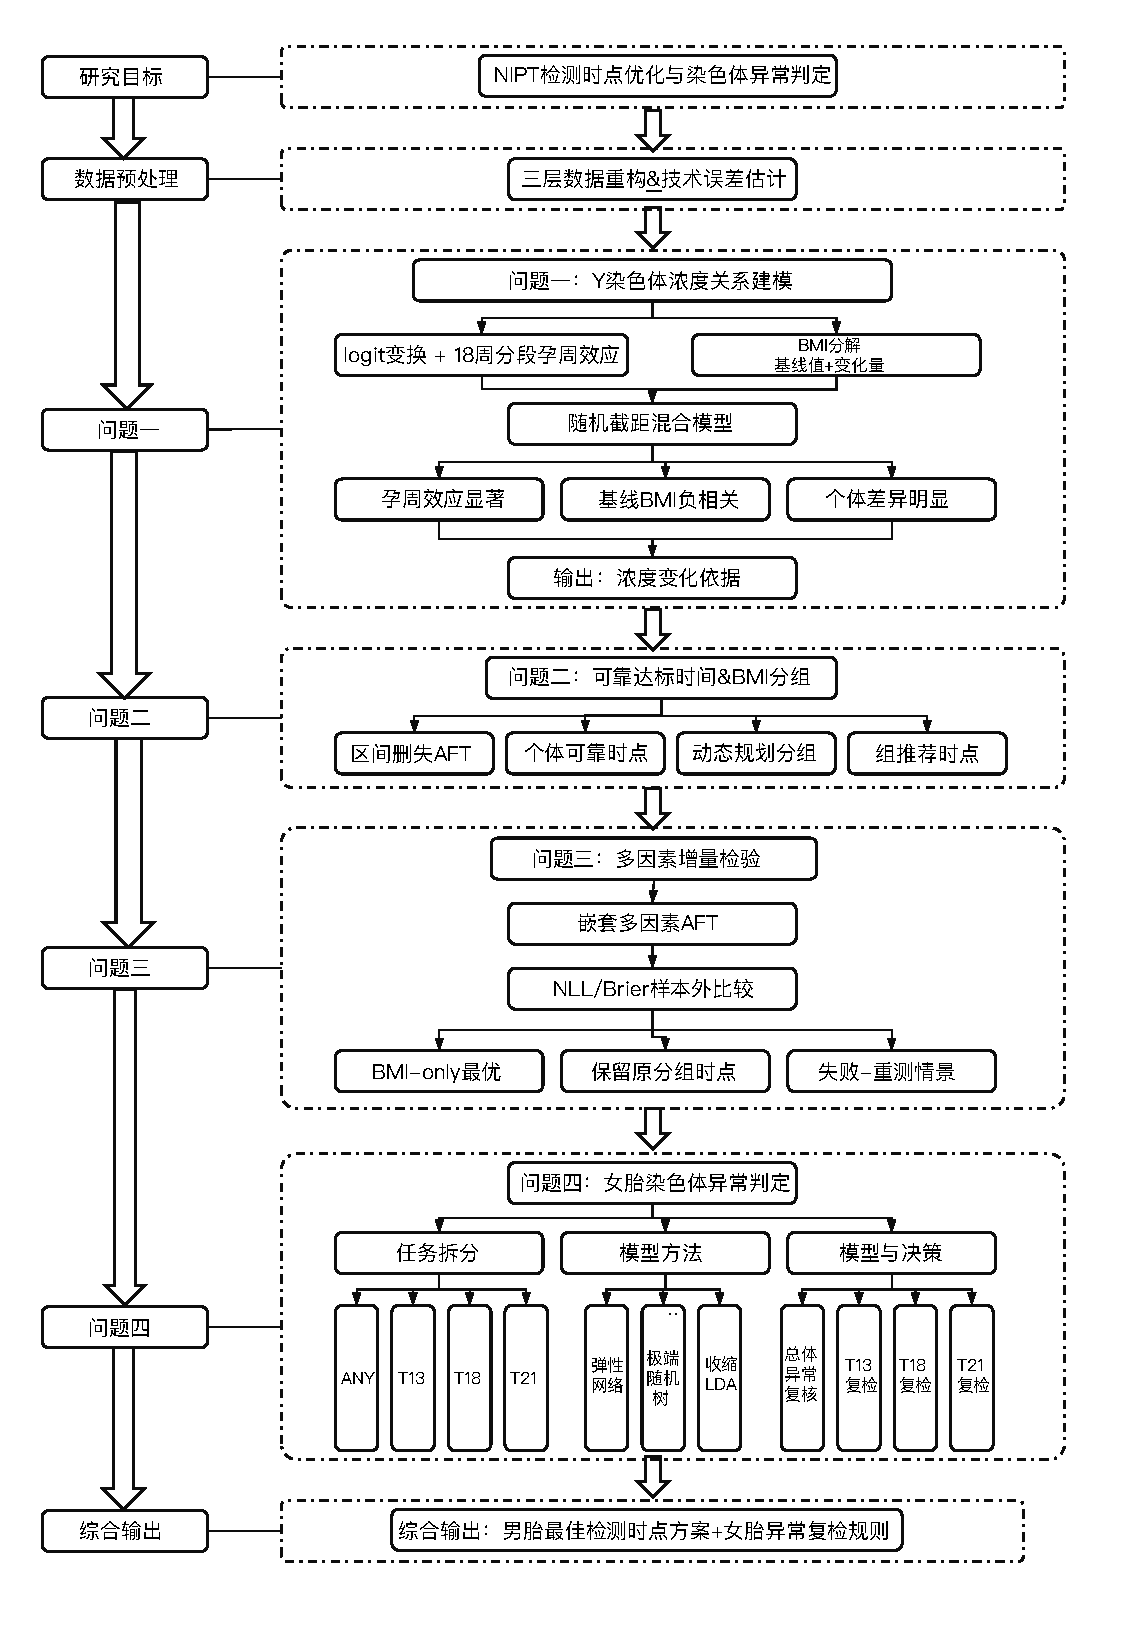
\includegraphics[
    width=\textwidth,
    height=0.86\textheight,
    keepaspectratio
  ]{figures/fig01_technical_route_bw.pdf}
  \caption{NIPT 检测时点优化与染色体异常判定的技术路线}
  \label{fig:workflow}
\end{figure}

\begin{table}[!htbp]
  \centering
  \caption{四个问题的输入、数学模型与输出}
  \label{tab:model-chain}
  \normalsize
  \setlength{\tabcolsep}{5pt}
  \renewcommand{\arraystretch}{1.55}
  \begin{tabularx}{\textwidth}{@{}Q{1.35cm}P{3.45cm}P{5.20cm}X@{}}
    \toprule
    问题 & 主要输入 & 数学模型 & 输出 \\
    \midrule
    问题一 & 孕周、基线 BMI、BMI 变化、Y 浓度 & 分段线性随机截距混合模型 & 孕周效应、BMI 效应、个体差异 \\
    问题二 & 达标区间、BMI、技术误差 & 区间删失 AFT 与一维动态规划 & BMI 切点、两档推荐时点 \\
    问题三 & 检测前个体特征、失败概率 & 嵌套多因素 AFT 与情景风险 & 分组修订结论、重测延迟 \\
    问题四 & Z 值、X 浓度、GC、读段、孕妇特征 & 弹性网络逻辑回归、极端随机树、收缩线性判别分析 & 总体异常筛查、分型概率、复检规则 \\
    \bottomrule
  \end{tabularx}
\end{table}

\section{3
模型假设与符号说明}\label{ux6a21ux578bux5047ux8bbeux4e0eux7b26ux53f7ux8bf4ux660e}

\subsection{3.1 模型假设}\label{ux6a21ux578bux5047ux8bbe}

为使数据结构、浓度达标和异常筛查具有统一的数学表达，作如下假设。

\begin{enumerate}
\def\labelenumi{\arabic{enumi}.}
\tightlist
\item
  同一孕妇、同一采血次数与近似相同孕周对应同一采血事件。该事件内的浓度差异主要来自技术复测波动。
\item
  孕妇间的随机效应相互独立，同一孕妇的多次访视在给定随机效应后满足模型规定的条件分布。
\item
  孕妇的首次可靠达标时间在观测区间内保持唯一。阈值上下的短期波动由技术误差和敏感性分析处理。
\item
  对数达标时间的分布可由对数正态、对数逻辑斯谛或 Weibull
  分布近似，具体分布由区间似然与信息准则选择。
\item
  女胎 AB 字段按题意视为监督标签。T13、T18 和 T21
  为可共存的二元标签，同一记录可以对多个染色体取值 1。
\end{enumerate}

\subsection{3.2 主要符号}\label{ux4e3bux8981ux7b26ux53f7}

表~\ref{tab:symbols} 汇总全文反复使用的主要符号。

\begin{table}[!htbp]
  \centering
  \caption{主要符号及其含义}
  \label{tab:symbols}
  \scriptsize
  \setlength{\tabcolsep}{5pt}
  \renewcommand{\arraystretch}{1.05}
  \begin{tabularx}{\textwidth}{@{}Q{3.3cm}X@{}}
    \toprule
    符号 & 含义 \\
    \midrule
    \(i=1,\ldots,n\) & 孕妇编号 \\
    \(v=1,\ldots,m_i\) & 孕妇 \(i\) 的采血访视编号 \\
    \(r=1,\ldots,R_{iv}\) & 采血事件 \((i,v)\) 内的技术记录编号 \\
    \(GA_{iv}\) & 采血事件 \((i,v)\) 的孕周 \\
    \(Y_{ivr}\) & 男胎检测记录的 Y 染色体浓度 \\
    \(\widetilde Y_{iv}\) & 同次采血复测浓度的稳健聚合值 \\
    \(B_{i0}\) & 孕妇 \(i\) 首次记录的 BMI \\
    \(\Delta B_{iv}\) & 当次 BMI 与 \(B_{i0}\) 之差 \\
    \(c\) & Y 染色体浓度达标阈值，\(c=0.04\) \\
    \(\sigma_{tech}\) & 同次采血复测估计的技术标准差 \\
    \(a(R_{iv})\) & \(R_{iv}\) 次技术复测中位数的标准误缩放因子 \\
    \(s_{iv,tech}\) & 采血事件 \((i,v)\) 聚合浓度的技术标准误 \\
    \(T_i\) & 孕妇 \(i\) 的首次达标时间 \\
    \((L_i,R_i]\) & \(T_i\) 的左、右删失边界 \\
    \(F_i(t)\) & 给定个体特征时 \(T_i\) 的分布函数 \\
    \(\rho\) & 时点政策的达标可靠度，主分析取 0.80 与 0.90 \\
    \(\tau_i(\rho)\) & 孕妇 \(i\) 在可靠度 \(\rho\) 下的个体达标时点 \\
    \(G_k\) & 第 \(k\) 个 BMI 连续分组 \\
    \(t_k\) & 组 \(G_k\) 的推荐检测时点 \\
    \(y_{rk}\) & 女胎记录 \(r\) 对染色体 \(k\) 的异常标签 \\
    \(p_{rk}\) & 女胎记录 \(r\) 对染色体 \(k\) 的异常概率 \\
    \(w_{ir}\) & 孕妇 \(i\) 的第 \(r\) 条记录权重 \\
    \(\theta_k\) & 女胎任务 \(k\) 的分类阈值 \\
    \bottomrule
  \end{tabularx}
\end{table}

\section{4
数据整理与测量误差}\label{ux6570ux636eux6574ux7406ux4e0eux6d4bux91cfux8befux5dee}

\subsection{4.1
样本构成与统计单位}\label{ux6837ux672cux6784ux6210ux4e0eux7edfux8ba1ux5355ux4f4d}

男胎数据包含 1082 条检测记录，对应 267 名孕妇和 1022
个采血访视事件。女胎数据包含 605 条记录，对应 147 名孕妇。表~\ref{tab:sample-structure}
给出与后续模型直接相关的数据构成。

\begin{table}[!htbp]
  \centering
  \caption{男胎、女胎与技术复测样本构成}
  \label{tab:sample-structure}
  \small
  \begin{tabularx}{\textwidth}{@{}P{3.0cm}Q{2.2cm}Q{2.2cm}X@{}}
    \toprule
    数据部分 & 检测记录数 & 孕妇数 & 关键结构 \\
    \midrule
    男胎 & 1082 & 267 & 1022 个采血访视，可构造纵向浓度和达标区间 \\
    女胎 & 605 & 147 & AB 为可共存多标签，多名孕妇有重复检测 \\
    男胎技术复测 & 39 组 & 按孕妇分组 & 组内差分自由度 60 \\
    严格日期复测 & 18 组 & 按孕妇分组 & 用于复核采血事件的定义 \\
    \bottomrule
  \end{tabularx}
\end{table}

表~\ref{tab:sample-structure} 给出统计单位，图~\ref{fig:gestational-atlas} 进一步检查孕周方向的观测支持。箱线图展示各孕周的浓度和原始读段分布，线性堆叠柱状图以总柱高表示采血事件数，并把其中达到 4\% 的事件单独着色，因而可以同时比较周际样本量与达标构成。山脊曲线给出六个 BMI 分位组的浓度形态。各组在主要检测窗口内均有观测，BMI 高位组在部分孕周的支持相对稀疏。

\begin{figure}[!htbp]
  \centering
  \includegraphics[page=5,width=\textwidth]{NIPT_真实数据参考组图复现.pdf}
  \caption{Y 染色体浓度、测序质量与 BMI 分层的孕周分布结构}
  \label{fig:gestational-atlas}
\end{figure}

对同一采血事件的多条复测，用中位数聚合 Y 染色体浓度：

\[
\widetilde Y_{iv}
=\operatorname{median}_{1\le r\le R_{iv}}Y_{ivr}.
\tag{1}
\]

中位数对个别异常检测值的敏感程度较低。采血事件层的孕周和 BMI
同样使用组内稳健中心，避免技术复测改变孕妇的实际随访次数。

\subsection{4.2
技术误差估计}\label{ux6280ux672fux8befux5deeux4f30ux8ba1}

设共有 \(G\) 个含技术复测的采血事件，第 \(g\) 组有 \(R_g\)
条记录，组内平均浓度为 \(\bar Y_g\)。技术方差用组内离差平方和估计：

\[
\widehat\sigma_{tech}^{2}
=
\frac{
\displaystyle\sum_{g=1}^{G}\sum_{r=1}^{R_g}
(Y_{gr}-\bar Y_g)^2
}{
\displaystyle\sum_{g=1}^{G}(R_g-1)
}.
\tag{2}
\]

估计得到

\[
\widehat\sigma_{tech}=0.0061265.
\tag{3}
\]

以孕妇为抽样单位进行 500 次 Bootstrap 重抽样，技术标准差的 95\% 置信区间为
\([0.0050516,0.0074917]\)，中位估计为 0.0061265。若在定义采血事件时同时要求检测日期相同，即仅将同日复测视为同一事件，则技术标准差估计值为
0.0047336。两种定义下的估计值差异不大，前者基于更多复测组，估计更稳定，故作为主分析结果；后者作为稳健性检验的参照。

技术标准差约为 0.61 个百分点，相对 4\%
的达标阈值不可忽略。一条观测浓度刚好高于 4\%
时，其对应的真实浓度仍可能位于阈值以下。这一结果将在问题二中通过浓度扰动和个体保守分位时点传递到推荐方案。

式（3）描述单条检测记录的技术波动。采血事件使用复测中位数后，其技术标准误随复测次数缩小。正态误差假设下，采用中位数的有限样本标准误因子

\[
a(R)=
\begin{cases}
1, & R=1,\\
2^{-1/2}, & R=2,\\
0.67017, & R=3,\\
\sqrt{\pi/(2R)}, & R\ge4,
\end{cases}
\qquad
\widehat s_{iv,tech}=\widehat\sigma_{tech}a(R_{iv}).
\tag{3a}
\]

该换算保留单次检测的完整误差，并反映技术复测对聚合浓度精度的改善。

\subsection{4.3
达标状态与删失类型}\label{ux8fbeux6807ux72b6ux6001ux4e0eux5220ux5931ux7c7bux578b}

达标判定规则为 \(\widetilde Y_{iv}\ge0.04\)。男胎 267
名孕妇中，217 名在首次有效访视时已达标，对应左删失；43
名孕妇在两次访视之间首次达标，对应区间删失；7
名孕妇至末次观测仍未达标，对应右删失。这一构成说明简单删除首次已达标样本会损失大部分数据，区间删失似然需同时容纳三类观测。

为表示阈值附近的测量不确定性，再定义基于置信区间的三状态判定。对采血事件的聚合浓度，取
\(z_{0.975}=1.96\)：

\[
S_{iv}=
\begin{cases}
1, & \widetilde Y_{iv}-1.96\widehat s_{iv,tech}\ge c,\\
0, & \widetilde Y_{iv}+1.96\widehat s_{iv,tech}<c,\\
?, & \text{其余情形}.
\end{cases}
\tag{4}
\]

其中 \(S_{iv}=1\) 表示可靠达标，\(S_{iv}=0\) 表示可靠未达标，\(?\)
表示阈值附近的不确定访视。基于该判定规则，267 名男胎孕妇中，235
名因首次访视即可靠达标而记为左删失，16 名在两次可靠状态之间首次达标而记为区间删失，9
名至末次访视仍未达到可靠标准而记为右删失；另有 7
名孕妇的全部访视均落入不确定带，无法判定达标状态。

三状态规则仅用于敏感性分析，以检验达标判定方式对时间分布的影响；排程采用的最终时点来自点事件定义下经技术误差扰动后的个体
95\% 保守时点。

\subsection{4.4 BMI
与女胎标签的样本支持}\label{bmi-ux4e0eux5973ux80ceux6807ux7b7eux7684ux6837ux672cux652fux6301}

男胎首次 BMI 的观测范围为 20.7031 至 46.8750，中位数为 31.2883。5\% 与
95\% 分位数分别为 28.2711 和 37.1757。BMI 不低于 36 的孕妇有 20
名，不低于 40 的孕妇有 4 名，不低于 42 的孕妇有 2 名。高 BMI
尾部样本密度快速降低，最高组的时点区间和组成稳定性需单独报告。

女胎数据中，ANY、T13、T18 和 T21 阳性记录数分别为 67、23、46 和
13，对应的阳性孕妇数为 44、18、30 和 12。共有 43 名孕妇的 ANY
标签在多次检测中发生变化。这一特征支持使用记录级标签进行判定，同时在权重和数据划分中将孕妇作为基本单位。

\section{5 问题一：Y
染色体浓度的纵向关系}\label{ux95eeux9898ux4e00y-ux67d3ux8272ux4f53ux6d53ux5ea6ux7684ux7eb5ux5411ux5173ux7cfb}

\subsection{5.1 响应变量变换与 BMI
分解}\label{ux54cdux5e94ux53d8ux91cfux53d8ux6362ux4e0e-bmi-ux5206ux89e3}

Y 染色体浓度的观测值介于 0.0100 与 0.2342
之间，具有明确上下界。对采血事件层的聚合浓度作对数几率变换：

\[
Z_{iv}
=\operatorname{logit}(\widetilde Y_{iv})
=\log\frac{\widetilde Y_{iv}}{1-\widetilde Y_{iv}}.
\tag{5}
\]

变换后的线性预测可通过逆变换返回 \((0,1)\)
区间，也使系数具有对数几率尺度上的明确含义。

设孕妇 \(i\) 的首次 BMI 为 \(B_{i0}\)，访视 \(v\) 的 BMI 为
\(B_{iv}\)，则

\[
B_{iv}=B_{i0}+\Delta B_{iv},
\qquad
\Delta B_{iv}=B_{iv}-B_{i0}.
\tag{6}
\]

\(B_{i0}\) 表示孕妇间的体型差异，\(\Delta B_{iv}\)
表示同一孕妇相对首次记录的变化。如果仅使用当次
BMI，两种效应会被压缩为同一回归系数。式（6）使后续分析能够直接回答``高
BMI 孕妇的浓度是否较低''，也能检查孕期内体重变化是否与浓度同步。

图~\ref{fig:gc-y-paths} 将四个 BMI 组的采血事件按孕周分箱，在相同坐标范围内连接相邻分箱的 GC 含量与 Y 染色体浓度中位数。颜色表示孕周，箭头表示局部推进方向。高 BMI 组的轨迹整体位于较低浓度区域，而四组轨迹都存在随孕周变化的局部回环，这为同时纳入孕周主效应和 BMI 分层效应提供了直观依据。

\begin{figure}[!htbp]
  \centering
  \includegraphics[page=2,width=\textwidth]{NIPT_真实数据参考组图复现.pdf}
  \caption{四个 BMI 组随孕周推进的 GC 含量与 Y 染色体浓度有序轨迹}
  \label{fig:gc-y-paths}
\end{figure}

\subsection{5.2
分段线性随机截距混合模型}\label{ux5206ux6bb5ux7ebfux6027ux968fux673aux622aux8dddux6df7ux5408ux6a21ux578b}

散点关系与分段斜率比较显示，18 周前后的孕周效应存在变化。定义正部函数

\[
(x)_+=\max(x,0),
\tag{7}
\]

孕周中心化为 \(GA_{iv}^{c}=GA_{iv}-16.6714\)。基线 BMI 中心化为
\(B_{i0}^{c}=B_{i0}-31.8261\)。问题一的主模型为

\[
\begin{aligned}
Z_{iv}={}&\beta_0+\beta_1GA_{iv}^{c}
+\beta_2B_{i0}^{c}
+\beta_3\Delta B_{iv}\\
&+\beta_4(GA_{iv}-18)_+
+u_i+\varepsilon_{iv},
\end{aligned}
\tag{8}
\]

其中

\[
u_i\sim N(0,\sigma_u^2),
\qquad
\varepsilon_{iv}\sim N(0,\sigma_e^2),
\qquad
u_i\perp\varepsilon_{iv}.
\tag{9}
\]

\(u_i\) 表示孕妇 \(i\) 相对人群平均水平的浓度偏移。在 18
周前，孕周斜率为 \(\beta_1\)；18 周后，斜率变为
\(\beta_1+\beta_4\)。该写法保证效应曲线在 18
周连续，同时允许增长速度改变。

对新孕妇计算人群平均预测时，取 \(u_i=0\)，再作逆对数几率变换：

\[
\widehat Y_{iv}
=\frac{\exp(\widehat Z_{iv})}
{1+\exp(\widehat Z_{iv})}.
\tag{10}
\]

对式（10）求导，可将对数几率尺度上的分段斜率还原为浓度尺度上的边际变化。除折点处外，孕周与基线
BMI 的边际效应分别为

\[
\frac{\partial \widehat Y_{iv}}{\partial GA_{iv}}
=\widehat Y_{iv}(1-\widehat Y_{iv})
\left[\widehat\beta_1+
\widehat\beta_4\mathbf 1(GA_{iv}>18)\right],
\tag{10a}
\]

\[
\frac{\partial \widehat Y_{iv}}{\partial B_{i0}}
=\widehat Y_{iv}(1-\widehat Y_{iv})\widehat\beta_2.
\tag{10b}
\]

因子 \(\widehat Y_{iv}(1-\widehat Y_{iv})\)
随当前浓度改变，因此相同的对数几率斜率在不同浓度水平下对应不同的绝对增量。18
周处预测曲线连续，左右导数分别由 \(\widehat\beta_1\) 和
\(\widehat\beta_1+\widehat\beta_4\) 决定。

\subsection{5.3
参数估计与关系解释}\label{ux53c2ux6570ux4f30ux8ba1ux4e0eux5173ux7cfbux89e3ux91ca}

表~\ref{tab:q1-fixed-effects}
给出混合模型的固定效应。系数的重抽样区间以孕妇为抽样单位，同一孕妇的全部访视在一次抽样中整体保留。

\begin{table}[!htbp]
  \centering
  \caption{分段线性随机截距混合模型的固定效应估计}
  \label{tab:q1-fixed-effects}
  \scriptsize
  \setlength{\tabcolsep}{3.2pt}
  \begin{tabularx}{\textwidth}{@{}Q{1.25cm}Q{1.55cm}Q{1.55cm}Q{1.65cm}Q{3.0cm}X@{}}
    \toprule
    参数 & 估计值 & 标准误 & \(p\) 值 & 95\% 重抽样区间 & 含义 \\
    \midrule
    \(\beta_0\) & -2.629790 & 0.030105 & \(<10^{-6}\) & [-2.686221, -2.569762] & 中心化参考个体的对数几率 \\
    \(\beta_1\) & 0.023380 & 0.005204 & \(7.0\times10^{-6}\) & [0.012938, 0.033802] & 18 周前每增加 1 周的孕周效应 \\
    \(\beta_2\) & -0.037978 & 0.009279 & \(4.3\times10^{-5}\) & [-0.057269, -0.015277] & 基线 BMI 的孕妇间效应 \\
    \(\beta_3\) & 0.012944 & 0.014341 & 0.366749 & [-0.020702, 0.043216] & 孕期内 BMI 变化的组内效应 \\
    \(\beta_4\) & 0.039769 & 0.009033 & \(1.1\times10^{-5}\) & [0.020896, 0.058667] & 18 周后的新增斜率 \\
    \(\beta_1+\beta_4\) & 0.063148 & --- & --- & [0.050117, 0.075137] & 18 周后的总孕周斜率 \\
    \bottomrule
  \end{tabularx}
\end{table}

18 周前每增加 1 周，Y 浓度对应几率乘以

\[
\exp(0.023380)=1.02366.
\tag{11}
\]

18 周后的周几率比为

\[
\exp(0.063148)=1.06519.
\tag{12}
\]

浓度在后一阶段的增长速度明确加快。将无折点的线性孕周模型与式（8）比较，似然比统计量为
19.1097，\(p=1.23\times10^{-5}\)，分段线性效应得到数据支持。

基线 BMI 每增加 1 个单位，Y 浓度对应几率乘以

\[
\exp(-0.037978)=0.96273.
\tag{13}
\]

在相同孕周下，基线 BMI 较高的孕妇具有较低的 Y
染色体浓度。\(\Delta B_{iv}\) 的区间跨越 0，孕期内 BMI
短期变化对浓度的独立关系较弱。问题一的 BMI 结论因而以基线 BMI
的孕妇间效应为主，这与后续使用首次 BMI 建立检测时点规则保持一致。

图~\ref{fig:q1-changepoint} 从序列检验与分段均值两个角度检查折点位置。浓度序列和 4\% 达标率的最小二乘变点分别位于 19 周和 16 周，18 周处于两类响应共同变化的过渡区；Mann--Kendall 顺序统计量也在该区间附近改变相对位置。综合连续响应、达标响应和参数简洁性，主模型采用 18 周作为统一的折点。

\begin{figure}[!htbp]
  \centering
  \includegraphics[page=6,width=\textwidth]{NIPT_真实数据参考组图复现.pdf}
  \caption{周内中位浓度与达标率的 Mann--Kendall 序列检验及分段变点比较}
  \label{fig:q1-changepoint}
\end{figure}

\subsection{5.4
孕妇间差异与典型效应曲线}\label{ux5b55ux5987ux95f4ux5deeux5f02ux4e0eux5178ux578bux6548ux5e94ux66f2ux7ebf}

随机截距方差为 0.182538，残差方差为 0.067359。同一孕妇内的组内相关系数为

\[
ICC
=\frac{\widehat\sigma_u^2}
{\widehat\sigma_u^2+\widehat\sigma_e^2}
=\frac{0.182538}{0.182538+0.067359}
=0.730454.
\tag{14}
\]

组内相关系数为 0.730454，表明约 73.0\% 的对数几率残余变异与孕妇间稳定差异相关。即便处于同一 BMI
组，个体达标时间仍存在明显的变异性。问题二则应基于达标时间分布开展计算。

表~\ref{tab:q1-predicted-y} 给出 BMI 为 28、32、36 和 40
时的人群平均预测。计算时取人群平均随机效应 \(u_i=0\)，并令
\(\Delta B=0\)。

\begin{table}[!htbp]
  \centering
  \caption{不同基线 BMI 与孕周组合下的预测 Y 染色体浓度}
  \label{tab:q1-predicted-y}
  \small
  \begin{tabularx}{0.92\textwidth}{@{}Q{2.1cm}*{5}{C}@{}}
    \toprule
    基线 BMI & 12 周 & 16 周 & 18 周 & 20 周 & 24 周 \\
    \midrule
    28 & 0.0695 & 0.0758 & 0.0792 & 0.0889 & 0.1116 \\
    32 & 0.0603 & 0.0659 & 0.0688 & 0.0773 & 0.0974 \\
    36 & 0.0523 & 0.0571 & 0.0597 & 0.0672 & 0.0848 \\
    40 & 0.0452 & 0.0495 & 0.0517 & 0.0583 & 0.0738 \\
    \bottomrule
  \end{tabularx}
\end{table}

四条曲线都随孕周上升，同一孕周的预测浓度则随 BMI 增大而降低。例如，12
周时 BMI=28 的预测值为 6.95\%，BMI=40 的预测值为 4.52\%。到 24
周时，两者分别为 11.16\% 和 7.38\%。BMI
的差异不仅改变某一孕周的预测浓度，还会通过阈值穿越改变达标时间的右尾。

图 \ref{fig:q1-joint} 将事件密度、边缘分布与模型曲线置于同一坐标系。图
\ref{fig:q1-surface} 按“模型响应—真实观测—分层达标”展开三维诊断。左图仅在孕周与
BMI 的样本凸包内绘制响应面，并将浓度等值线投影到底面；中图保留 1011
次男胎采血事件及 4\% 阈值面；右图将事件汇总为整孕周与四个 BMI 政策组的达标率柱阵，
并以叉号标记样本量小于 5 的单元。

\begin{figure}[!htbp]
\centering
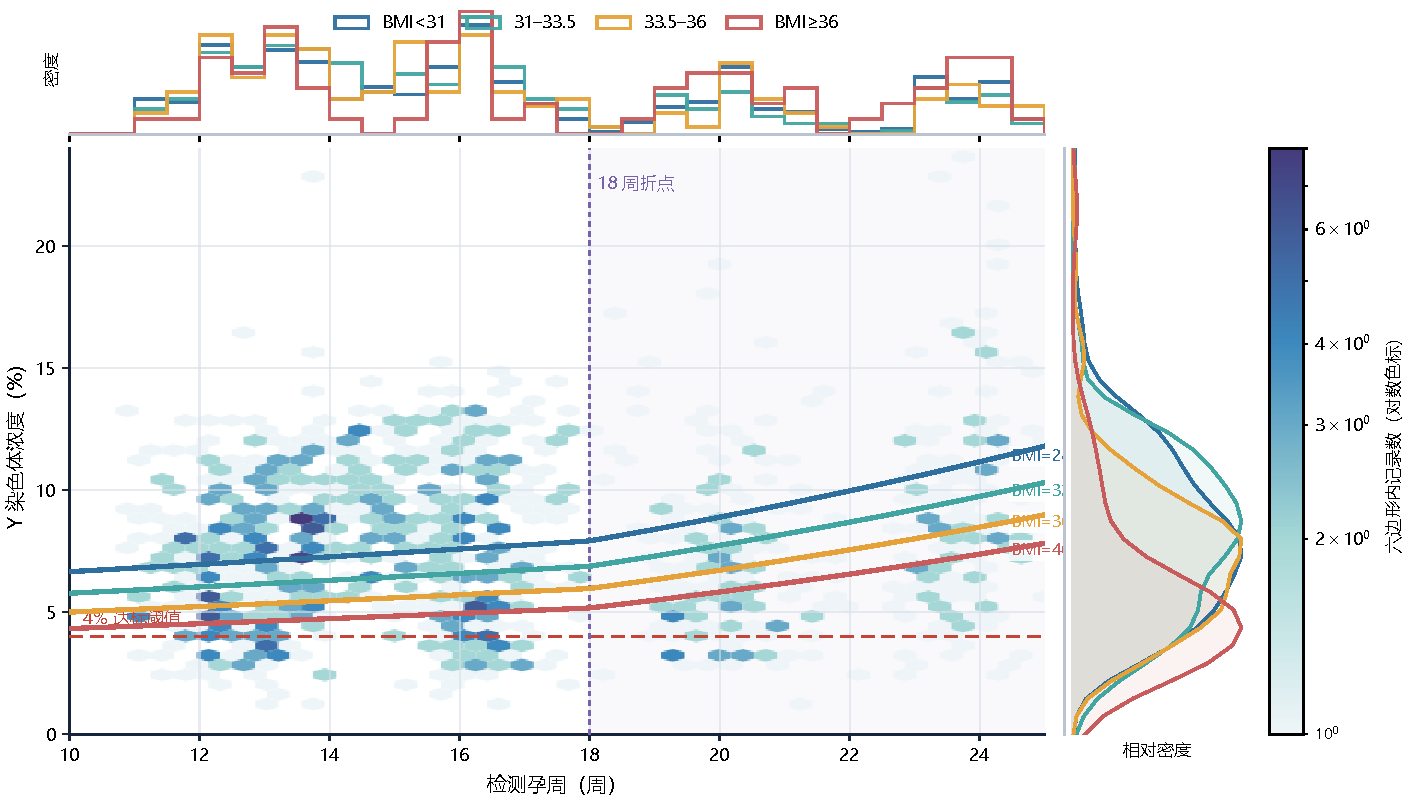
\includegraphics[width=0.98\textwidth]{figures/fig02_q1_joint_density.pdf}
\caption{孕周—Y 染色体浓度的事件密度、BMI 分层曲线与边缘分布}
\label{fig:q1-joint}
\end{figure}

\begin{figure}[!htbp]
\centering
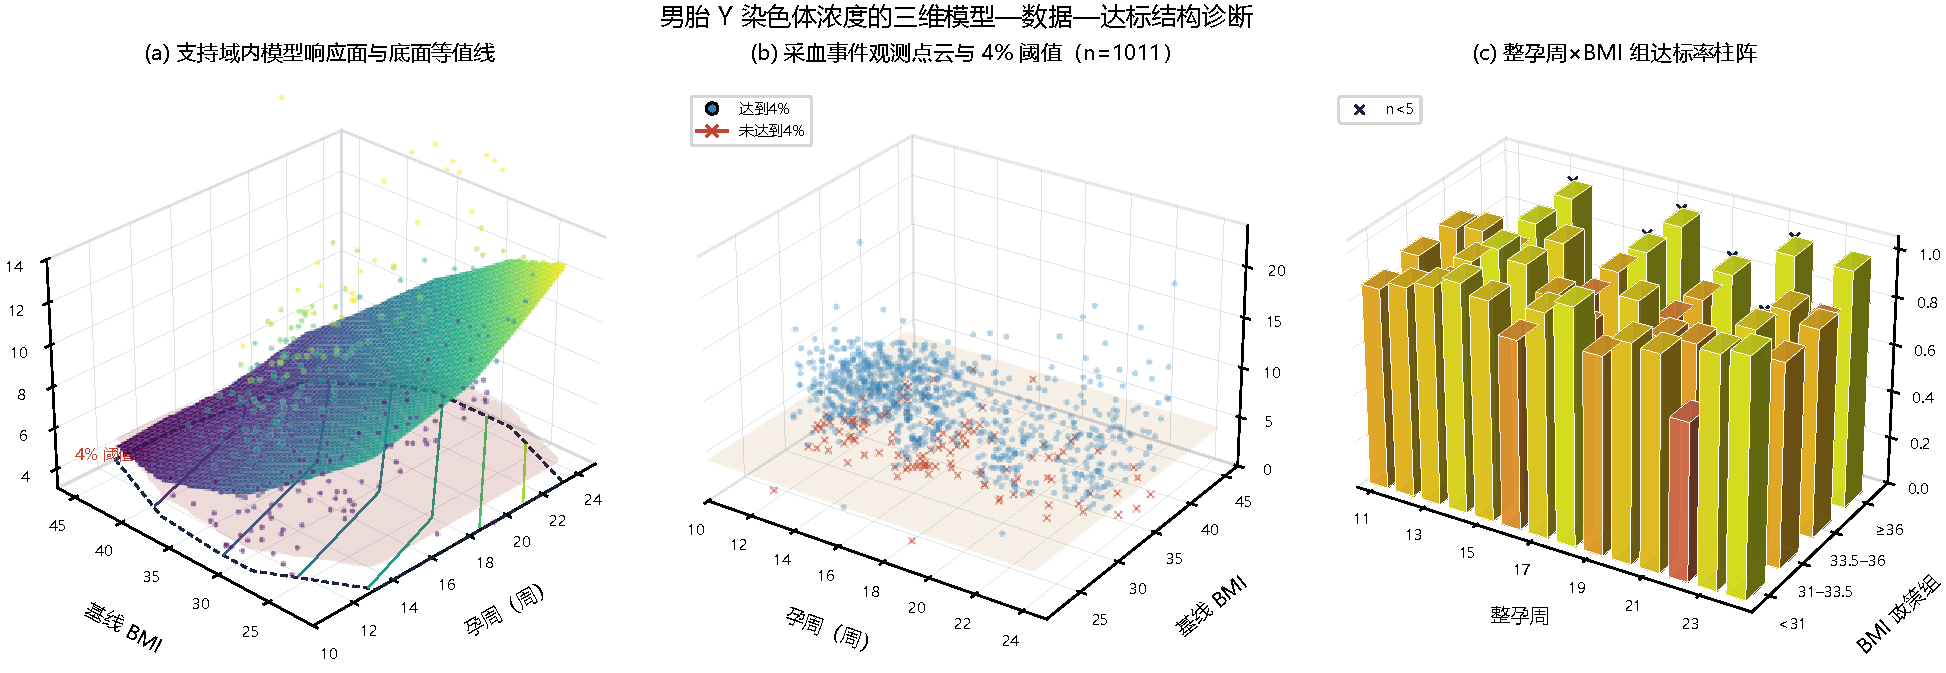
\includegraphics[width=\textwidth]{figures/fig03_q1_response_surface.pdf}
\caption{男胎 Y 染色体浓度的三维模型响应、观测点云与分层达标结构}
\label{fig:q1-surface}
\end{figure}

\subsection{5.5
预测比较与机器学习辅助}\label{ux9884ux6d4bux6bd4ux8f83ux4e0eux673aux5668ux5b66ux4e60ux8f85ux52a9}

该混合模型对孕周、基线 BMI、组内 BMI
变化与孕妇间差异进行分解。在统一的孕妇级划分条件下，对比线性混合模型、分段线性混合模型、岭回归和随机森林，评估局部非线性对浓度预测的作用差异。同一孕妇的记录在每次划分中保持同组。表~\ref{tab:q1-model-comparison} 汇总四种模型的样本外均方根误差（RMSE）、平均绝对误差（MAE）与决定系数
\(R^2\)。

\begin{table}[!htbp]
  \centering
  \caption{男胎 Y 染色体浓度模型的孕妇级样本外预测性能}
  \label{tab:q1-model-comparison}
  \small
  \begin{tabularx}{\textwidth}{@{}P{4.2cm}Q{1.8cm}Q{1.8cm}Q{1.8cm}X@{}}
    \toprule
    模型 & RMSE & MAE & \(R^2\) & 主要用途 \\
    \midrule
    线性混合模型 & 0.03378 & 0.02737 & -0.0524 & 线性参照 \\
    18 周分段线性混合模型 & 0.03389 & 0.02741 & -0.0595 & 关系解释与个体差异估计 \\
    岭回归 & 0.03254 & 0.02636 & 0.0251 & 正则化线性预测参照 \\
    随机森林 & 0.03099 & 0.02450 & 0.1176 & 局部非线性预测 \\
    \bottomrule
  \end{tabularx}
\end{table}

线性与分段线性混合模型的 RMSE 相差
0.00011，点预测差异很小。似然比检验确认了 18
周前后的斜率改变，关系解释因此采用分段线性混合模型。局部浓度预测中，随机森林相对岭回归将
RMSE 降低 4.762\%。配对改善量的 95\% 区间为
\([0.001179,0.001817]\)，全部重复划分呈现同一方向。随机森林用于补充浓度点预测；参数解释、外推趋势以及问题二的时间分布仍然依托统计模型实现。

图~\ref{fig:q1-longitudinal-dashboard} 将主模型的纵向浓度形态、周内达标进程、BMI 样本支持和 BMI 校正残差置于同一页。十个首次 BMI 分位组的局部回归曲线保持共同上升趋势，高 BMI 组整体偏低；校正残差没有形成随 BMI 分位组单调扩大的系统偏移。该图把表~\ref{tab:q1-fixed-effects} 的参数结论与样本层面的浓度变化对应起来。

\begin{figure}[!htbp]
  \centering
  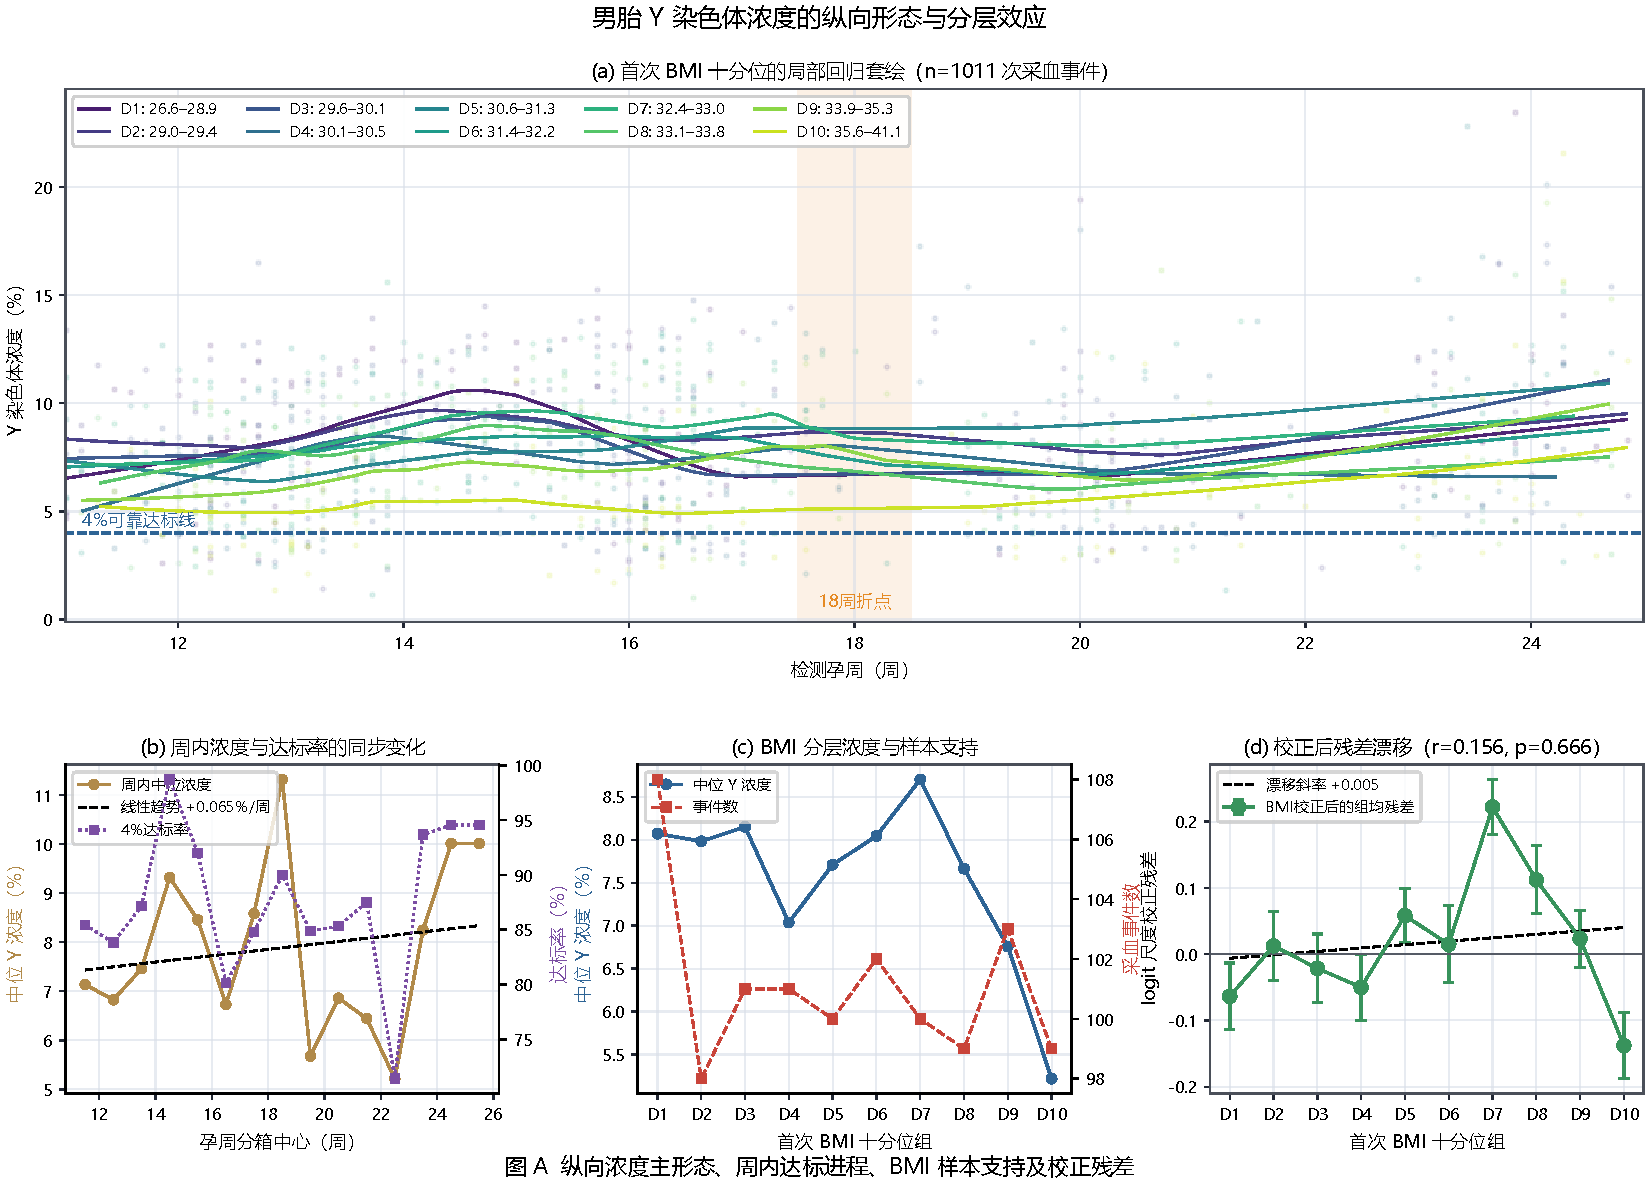
\includegraphics[page=1,width=\textwidth]{NIPT_真实数据参考组图复现.pdf}
  \caption{男胎 Y 染色体浓度的纵向形态、达标进程、BMI 样本支持与校正残差}
  \label{fig:q1-longitudinal-dashboard}
\end{figure}

\subsection{5.6 问题一结论}\label{ux95eeux9898ux4e00ux7ed3ux8bba}

男胎 Y 染色体浓度随孕周上升，18 周后的上升速度较快。18
周前后的对数几率周斜率分别为 0.02338 和 0.06315。基线 BMI 系数为
-0.03798，高 BMI 孕妇在相同孕周下具有较低的预测浓度。孕期内 BMI
变化系数的区间跨越 0，基线 BMI 更适合用于后续分组。组内相关系数为
0.7305，说明个体差异是达标时间离散的重要来源。

浓度关系已给出问题二的两个建模依据：BMI
需要作为达标时间的主要分组变量，孕妇间的高异质性要用时间分布和保守分位点表示。

\FloatBarrier

\section{6 问题二：可靠达标时间与 BMI
分组}\label{ux95eeux9898ux4e8cux53efux9760ux8fbeux6807ux65f6ux95f4ux4e0e-bmi-ux5206ux7ec4}

\subsection{6.1
首次达标时间的区间表示}\label{ux9996ux6b21ux8fbeux6807ux65f6ux95f4ux7684ux533aux95f4ux8868ux793a}

设 \(T_i\) 为孕妇 \(i\) 的 Y 染色体浓度首次达到 4\%
的孕周。由于采血仅在离散的访视时间点进行，\(T_i\)
通常无法被直接观测，只能确定其落在两次检测之间。将每名孕妇的采血事件按孕周升序排列后，达标时间的删失区间按下式定义：

\[
(L_i,R_i]=
\begin{cases}
(0,t_{i1}], & \text{首次访视已达标},\\
(t_{i,j-1},t_{ij}], & t_{ij}\text{ 为首次达标访视},\\
(t_{im_i},+\infty), & \text{末次访视仍未达标}.
\end{cases}
\tag{15}
\]

式（15）将左删失、区间删失和右删失写成统一时间区间。217
个左删失样本保留了``达标时间早于首次检测''的信息，7
个右删失样本保留了时间分布的右尾。两类样本都会影响高分位时点，在稳健推荐中尤为重要。

三状态规则将落入不确定带的访视排除在达标状态判定之外。令 \(R_i\)
为首个可靠达标时点，\(L_i\)
为其前最近的可靠未达标时点，删失区间的边界仅由最近的可靠达标与可靠未达标时点确定。通过对比三状态口径与点事件口径的估计结果，可以判断阈值附近访视对达标时间推断的影响程度。

\subsection{6.2
区间删失加速失效时间模型}\label{ux533aux95f4ux5220ux5931ux52a0ux901fux5931ux6548ux65f6ux95f4ux6a21ux578b}

加速失效时间模型直接描述 BMI 对达标时间的倍率影响。对首次 BMI 作标准化：

\[
Z_{B,i}=\frac{B_{i0}-31.84744}{2.98614}.
\tag{16}
\]

对数正态模型写为

\[
\log T_i=\alpha_0+\alpha_B Z_{B,i}+\sigma\varepsilon_i,
\qquad
\varepsilon_i\sim N(0,1),
\quad \alpha_B\ge0.
\tag{17}
\]

\(\alpha_B\ge0\) 表示 BMI
增大不会系统性提前达标时间，该方向与问题一中基线 BMI 对 Y
浓度的负向关系一致。给定 BMI 时，\(T_i\) 的分布函数为

\[
F(t\mid B_{i0})
=\Phi\left[
\frac{\log t-\alpha_0-\alpha_B Z_{B,i}}{\sigma}
\right].
\tag{18}
\]

删失区间是对 \(T_i\) 的集合观测。将 \(F_i(t)=F(t\mid B_{i0})\)
代入区间概率，第 \(i\) 名孕妇的对数似然贡献为

\[
\ell_i=
\begin{cases}
\log F_i(R_i), & L_i=0,\\[4pt]
\log\{F_i(R_i)-F_i(L_i)\}, & 0<L_i<R_i<+\infty,\\[4pt]
\log\{1-F_i(L_i)\}, & R_i=+\infty.
\end{cases}
\tag{19}
\]

模型参数由下式估计：

\[
(\widehat\alpha_0,\widehat\alpha_B,\widehat\sigma)
=\arg\max_{\alpha_B\ge0,\,\sigma>0}
\sum_{i=1}^{n}\ell_i.
\tag{20}
\]

式（19）中的三项分别使用首次已达标、两次访视之间达标与访视结束时未达标的信息。所有孕妇均以可观测的时间集合参与估计，真实达标时间保持区间形式。

\subsection{6.3 分布选择与 BMI
时间比}\label{ux5206ux5e03ux9009ux62e9ux4e0e-bmi-ux65f6ux95f4ux6bd4}

为检查达标时间右尾的分布形态，在相同的 BMI
线性预测式下比较对数正态、对数逻辑斯谛和 Weibull 分布。表~\ref{tab:q2-distribution}
中三个模型的赤池信息准则（AIC）差异小于
0.6，对数正态分布取得最小值。表中同时列出贝叶斯信息准则（BIC）。对数正态分位时点有解析形式，且便于后续将
BMI 效应解释为时间比。

\begin{table}[!htbp]
  \centering
  \caption{首次达标时间候选分布的拟合比较}
  \label{tab:q2-distribution}
  \small
  \begin{tabularx}{0.92\textwidth}{@{}P{3.2cm}Q{2.0cm}Q{2.0cm}Q{2.6cm}X@{}}
    \toprule
    候选分布 & AIC & BIC & 估计尺度参数 & 模型位置 \\
    \midrule
    对数正态 & 368.0336 & 378.7954 & 0.53399 & 主模型 \\
    对数逻辑斯谛 & 368.5516 & 379.3134 & 0.27476 & 分布敏感性 \\
    Weibull & 368.4865 & 379.2483 & 0.70362 & 分布敏感性 \\
    \bottomrule
  \end{tabularx}
\end{table}

点事件定义下，对数正态模型为

\[
\log T_i
=2.04707
+0.11701\frac{B_{i0}-31.84744}{2.98614}
+0.53399\varepsilon_i.
\tag{21}
\]

将标准化系数换算到原 BMI 尺度，每增加 1 个 BMI 单位的时间比为

\[
TR_B
=\exp\left(\frac{\alpha_B}{2.98614}\right).
\tag{22}
\]

表~\ref{tab:q2-time-ratio} 给出不同误差定义下的时间比。点事件模型的重抽样中位数为 1.03977，即
BMI 每增加 1，达标时间按中位效应约延后 3.98\%。在 Y
浓度上加入技术扰动并重新构造事件后，中位时间比为 1.03308，其 95\%
区间上限为 1.07386。

\begin{table}[!htbp]
  \centering
  \caption{不同达标定义下 BMI 时间比的重抽样结果}
  \label{tab:q2-time-ratio}
  \small
  \begin{tabularx}{0.92\textwidth}{@{}P{3.2cm}Q{2.8cm}Q{4.0cm}X@{}}
    \toprule
    达标定义 & 时间比中位数 & 95\% 区间 & BMI 正向系数频率 \\
    \midrule
    点事件 & 1.03977 & [1.00704, 1.07322] & 99.6\% \\
    技术误差扰动 & 1.03308 & [1.00000, 1.07386] & 97.2\% \\
    三状态判定 & 1.08472 & [1.02020, 1.15833] & 99.4\% \\
    \bottomrule
  \end{tabularx}
\end{table}

三种口径对 BMI
效应的方向一致，效应幅度随阈值不确定性的处理而变化。这种幅度差异将通过个体保守时点体现在推荐结果中，分组方向保持为``BMI
越高，推荐时点越晚''。

\subsection{6.4
个体可靠时点与误差传递}\label{ux4e2aux4f53ux53efux9760ux65f6ux70b9ux4e0eux8befux5deeux4f20ux9012}

给定政策可靠度 \(\rho\)，孕妇 \(i\) 的个体达标时点定义为

\[
\tau_i(\rho)
=\inf\{t:F_i(t)\ge\rho\}.
\tag{23}
\]

对数正态 AFT 下，式（23）可写成

\[
\tau_i(\rho)
=\exp\left[
\alpha_0+\alpha_BZ_{B,i}
+\sigma\Phi^{-1}(\rho)
\right].
\tag{24}
\]

固定可靠度 \(\rho\) 后，两名基线 BMI 相差 \(\Delta B\)
的孕妇，其分位时点之比为

\[
\frac{\tau(\rho;B+\Delta B)}{\tau(\rho;B)}
=\exp\left(\frac{\alpha_B\Delta B}{2.98614}\right)
=TR_B^{\Delta B}.
\tag{24a}
\]

可靠度项 \(\sigma\Phi^{-1}(\rho)\)
在比值中相消。由此，可靠度控制时点的整体保守程度，BMI
时间比决定个体之间的相对推迟幅度。

\(\rho=0.80\) 表示在该时点前达标的模型概率为 80\%；\(\rho=0.90\)
使用更高的分位点，对应更保守的时点。

技术误差从参数估计继续传递至采血事件浓度、删失状态和推荐时点。第 \(b\)
次重抽样以孕妇为簇，并对采血事件层浓度施加扰动

\[
\widetilde Y_{iv}^{(b)}
=\min\left\{
1,\max\left(0,\widetilde Y_{iv}+e_{iv}^{(b)}\right)
\right\},
\qquad
e_{iv}^{(b)}\sim N(0,\widehat s_{iv,tech}^{\,2}).
\tag{25}
\]

每次扰动都重新判定达标状态、构造删失区间、估计 AFT 参数并计算
\(\tau_i^{(b)}(\rho)\)。个体保守时点取 500 次扰动结果的 95\% 分位数：

\[
\tau_i^{rob}(\rho)
=Q_{0.95}\left\{
\tau_i^{(1)}(\rho),\ldots,
\tau_i^{(500)}(\rho)
\right\}.
\tag{26}
\]

式（26）同时包含样本构成、阈值状态与 AFT 参数的波动。组推荐采用
\(\tau_i^{rob}(\rho)\)，把个体不确定性传递到组时点。

\subsection{6.5
组时点的严格覆盖约束}\label{ux7ec4ux65f6ux70b9ux7684ux4e25ux683cux8986ux76d6ux7ea6ux675f}

对任意一个 BMI 组 \(G\)，将组内个体保守时点按升序排列：

\[
\tau_{(1)}^{rob}
\le\tau_{(2)}^{rob}
\le\cdots
\le\tau_{(|G|)}^{rob}.
\tag{27}
\]

组推荐时点取上取整次序统计量：

\[
t_G(\rho)
=\tau_{(\lceil\rho|G|\rceil)}^{rob}.
\tag{28}
\]

由式（28）直接得到

\[
\frac{1}{|G|}
\sum_{i\in G}
\mathbf 1
\{\tau_i^{rob}(\rho)\le t_G(\rho)\}
\ge\rho.
\tag{29}
\]

上取整是覆盖约束成立的关键。若使用分位数的线性插值，推荐时点可能位于两个个体时点之间，实际满足约束的孕妇比例就会低于
\(\rho\)。

潜在风险由孕周划分为三档，对应的有序风险函数为

\[
r(t)=
\begin{cases}
1,&t\le 12,\\
2,&12<t\le 27,\\
3,&t>27.
\end{cases}
\tag{29a}
\]

对固定 BMI 组，满足式（29）的时点构成可行集合
\(\mathcal A_G(\rho)\)。式（28）正是该集合中的最早时点，即
\(t_G(\rho)=\inf\mathcal A_G(\rho)\)。由于 \(r(t)\)
随孕周不减，这个时点在满足可靠度后同时取得最低风险档；处于同一风险档时，较早孕周优先。于是，``潜在风险最小''被写成可靠度约束下的最早可行时点，题目给出的风险档次和连续孕周共同决定排程顺序。

\subsection{6.6 BMI
连续分组的动态规划}\label{bmi-ux8fdeux7eedux5206ux7ec4ux7684ux52a8ux6001ux89c4ux5212}

按首次 BMI 将孕妇排序：

\[
B_{(1)}\le B_{(2)}\le\cdots\le B_{(n)}.
\tag{30}
\]

将与 \(B_{(r)}\) 配对的个体保守时点记为
\(\tau_{[r]}^{rob}\)。方括号表示按 BMI
排序后的对应个体，与式（27）中按达标时点排序的圆括号相区别。每一组必须是序列中的连续区间，相同
BMI 的孕妇保持同组。候选组数取 \(K\in\{2,3,4,5,6\}\)，每组样本量不小于

\[
n_{min}=\max\{20,\lceil0.07n\rceil\}=20.
\tag{31}
\]

对任意候选连续段 \(i{:}j\)，依据式（28）计算段时点
\(t_{ij}\)。为衡量将个体时点压缩为组时点的损失，定义分位数损失

\[
\ell_{\rho}(u)
=u\left[\rho-\mathbf 1(u<0)\right],
\tag{32}
\]

候选段的代价为

\[
C(i,j)
=\sum_{r=i}^{j}
\ell_{\rho}
\left(\tau_{[r]}^{rob}-t_{ij}\right).
\tag{33}
\]

当某段需要的推荐时点超出 25
周时，将其标记为常规窗口内不可行。个体时点在计算中保留原值，不将超窗口时点截成
25 周。

令 \(DP(k,j)\) 表示前 \(j\) 名孕妇分为 \(k\) 个连续 BMI 组的最小损失，则

\[
DP(1,j)=C(1,j),
\tag{34}
\]

\[
DP(k,j)
=\min_{h}
\left\{
DP(k-1,h)+C(h+1,j)
\right\},
\tag{35}
\]

其中前一段和新段都需满足式（31）。记录每个状态的最优前驱后，从
\(DP(K,n)\) 回溯即可得到全局最优切分。候选段规模为
\(O(n^2)\)，整体递推复杂度为
\(O(Kn^2)\)，该递推枚举全部合法连续分组，直接给出全局最优值。

若最优分割位于 \(B_{(j)}\) 和 \(B_{(j+1)}\)
之间，原始切点取两者中点。为使规则易于使用，切点舍入到最近的 0.5 个 BMI
单位，并重新分配全部孕妇、重算组时点和覆盖率。舍入后的切点在式（29）仍成立时用于正式分组。

\subsection{6.7
组数选择与切点}\label{ux7ec4ux6570ux9009ux62e9ux4e0eux5207ux70b9}

组数增加会降低组内个体时点的异质性损失，同时提升分组规则的复杂度。基于技术误差重抽样的个体时点中位数计算损失，以
2 组至 6 组的最大可实现降幅为基准：\(\rho=0.80\) 时，4 组对应的损失降幅占比为
89.12\%；\(\rho=0.90\) 时占比为 92.68\%。组数从 4 组增至 5
组，损失降幅可额外提升 5.74 与 4.17
个百分点，同时新增一个切点，部分组样本量接近统计下限。

原始切点在两档 \(\rho\) 下都集中于 31、33.5 和 36
附近。舍入并重算后的规则为

\[
G(B)=
\begin{cases}
1, & B<31,\\
2, & 31\le B<33.5,\\
3, & 33.5\le B<36,\\
4, & B\ge36.
\end{cases}
\tag{36}
\]

四组样本量依次为 123、82、42 和 20。最高组正好达到最小组样本量，且 BMI
40 以上样本很少，因而高 BMI 尾部的推荐需结合区间宽度和超窗口个体数解释。

\subsection{\texorpdfstring{6.8
平衡方案：\(\rho=0.80\)}{6.8 平衡方案：\textbackslash rho=0.80}}\label{ux5e73ux8861ux65b9ux6848rho0.80}

表~\ref{tab:q2-rho80} 给出 80\%
可靠度下的四组结果。``点估计时点''来自式（24）和动态规划，``推荐时点''则取式（26）得到的个体保守时点并向上舍入到整天。

\begin{table}[!htbp]
  \centering
  \caption{80\% 可靠度下的 BMI 分组与推荐检测时点}
  \label{tab:q2-rho80}
  \scriptsize
  \setlength{\tabcolsep}{2.6pt}
  \begin{tabularx}{\textwidth}{@{}P{2.2cm}Q{1.0cm}Q{1.8cm}Q{2.7cm}Q{1.9cm}Q{1.9cm}X@{}}
    \toprule
    BMI 区间 & 人数 & 点估计时点 & 点时点 95\% 区间 & 推荐时点 & 平均达标概率 & 个体保守覆盖率 \\
    \midrule
    \(B<31\) & 123 & 11.770 周 & [10.000, 12.998] & 12 周+6 天 & 0.8572 & 0.9024 \\
    \(31\le B<33.5\) & 82 & 12.870 周 & [11.569, 14.115] & 14 周 & 0.8543 & 0.8780 \\
    \(33.5\le B<36\) & 42 & 13.894 周 & [11.992, 15.846] & 15 周+4 天 & 0.8662 & 0.8095 \\
    \(B\ge36\) & 20 & 15.871 周 & [12.483, 20.673] & 19 周+6 天 & 0.8937 & 0.8000 \\
    \bottomrule
  \end{tabularx}
\end{table}

四组的推荐时点随 BMI 递增，且都位于题目给定的 25
周窗口内。四组的平均达标概率在 0.8543 至 0.8937 之间，高于政策参数
0.80。个体保守覆盖率与组覆盖约束的定义更严，最高 BMI 组恰好为
0.80。该组的点时点区间宽度也最大，因而 19 周+6 天是对高 BMI
尾部的保守安排。

按式（29a）的风险分档，四组时点均超过 12 周低风险边界，且未超过 27
周，因而落在第二档。第 1 组超出低风险边界 6 天，第 4 组超出 7 周+6
天。可靠度约束使这些时点成为各组当前可达到的最早排程；降低技术误差或补充早孕期访视，才可能把更多孕妇的推荐时点推进到
12 周以内。

\subsection{\texorpdfstring{6.9
保守方案：\(\rho=0.90\)}{6.9 保守方案：\textbackslash rho=0.90}}\label{ux4fddux5b88ux65b9ux6848rho0.90}

当决策更重视一次检测已达标的概率时，取 \(\rho=0.90\)。表~\ref{tab:q2-rho90} 给出同一 BMI
分组下的时点。

\begin{table}[!htbp]
  \centering
  \caption{90\% 可靠度下的 BMI 分组与推荐检测时点}
  \label{tab:q2-rho90}
  \scriptsize
  \setlength{\tabcolsep}{2.4pt}
  \begin{tabularx}{\textwidth}{@{}P{2.2cm}Q{1.0cm}Q{1.8cm}Q{2.7cm}Q{1.9cm}Q{1.8cm}X@{}}
    \toprule
    BMI 区间 & 人数 & 点估计时点 & 点时点 95\% 区间 & 推荐时点 & 平均达标概率 & 窗口内处理 \\
    \midrule
    \(B<31\) & 123 & 14.843 周 & [13.082, 16.572] & 16 周+2 天 & 0.9361 & 按推荐时点检测 \\
    \(31\le B<33.5\) & 82 & 16.229 周 & [14.594, 18.216] & 17 周+6 天 & 0.9361 & 按推荐时点检测 \\
    \(33.5\le B<36\) & 42 & 17.557 周 & [14.951, 20.641] & 20 周+2 天 & 0.9464 & 按推荐时点检测 \\
    \(B\ge36\) & 20 & 21.128 周 & [15.339, 29.816] & 28 周+3 天 & 0.9695 & 25 周内无法统一保证，个体化复检 \\
    \bottomrule
  \end{tabularx}
\end{table}

前三组的保守时点位于 16 周+2 天至 20 周+2 天之间，平均达标概率都超过
0.93。BMI 不低于 36 的组中，7 名孕妇的个体 95\% 保守时点晚于 25
周。若组内 90\% 的组员可达到个体保守时点，组时点需推迟至 28 周+3
天，这处于晚期极高风险区间，且超出常规检测窗口。所以该组在
90\% 可靠度下采用个体化复检的方案，结合实际 Y 浓度调整后续检测时点。

图~\ref{fig:q2-timing-distribution} 把问题二的证据链集中在同一组图中：上部热图展示孕周与 BMI 组的周内中位浓度，并用青色窗口标出 80\% 可靠度下的推荐时点；下部雨云图和经验累积分布保留个体 95\% 保守时点，堆叠图则给出各组时点所处区间的成员构成。由个体分布到组时点的压缩过程因此能够直接核对。

\begin{figure}[!htbp]
  \centering
  \includegraphics[page=3,width=\textwidth]{NIPT_真实数据参考组图复现.pdf}
  \caption{BMI 分组下的浓度日历、个体保守时点分布与组内时点构成}
  \label{fig:q2-timing-distribution}
\end{figure}

\subsection{6.10
检测误差对时点的影响}\label{ux68c0ux6d4bux8befux5deeux5bf9ux65f6ux70b9ux7684ux5f71ux54cd}

技术误差会改变阈值附近访视的达标状态，继而改变删失区间和右尾分位点。各组时点的改变量并非常数。保守推荐与点估计之差随
BMI 增大，在 \(\rho=0.80\) 时四组分别约为 1.09、1.13、1.68 和 3.99
周。这一差异结合了参数波动和组内高分位成员，最高 BMI 组的延长最明显。

在 \(\rho=0.90\) 时，前三组的保守时点相对点估计分别推迟约 1.44、1.63 和
2.73 周。最高组的差异扩大到 7.30 周，对应点时点区间的上限 29.816
周。因此，对测量误差的处理直接改变了高 BMI
尾部的决策类型：从统一排程转为常规窗口内的个体化复检。

图~\ref{fig:q2-sensitivity} 同时展示候选组数的损失变化与达标阈值扰动下的时点移动。四组方案位于复杂度继续增加而边际收益趋缓的位置；阈值上调时，各组推荐时点整体后移，分组次序保持不变。

\begin{figure}[!htbp]
\centering
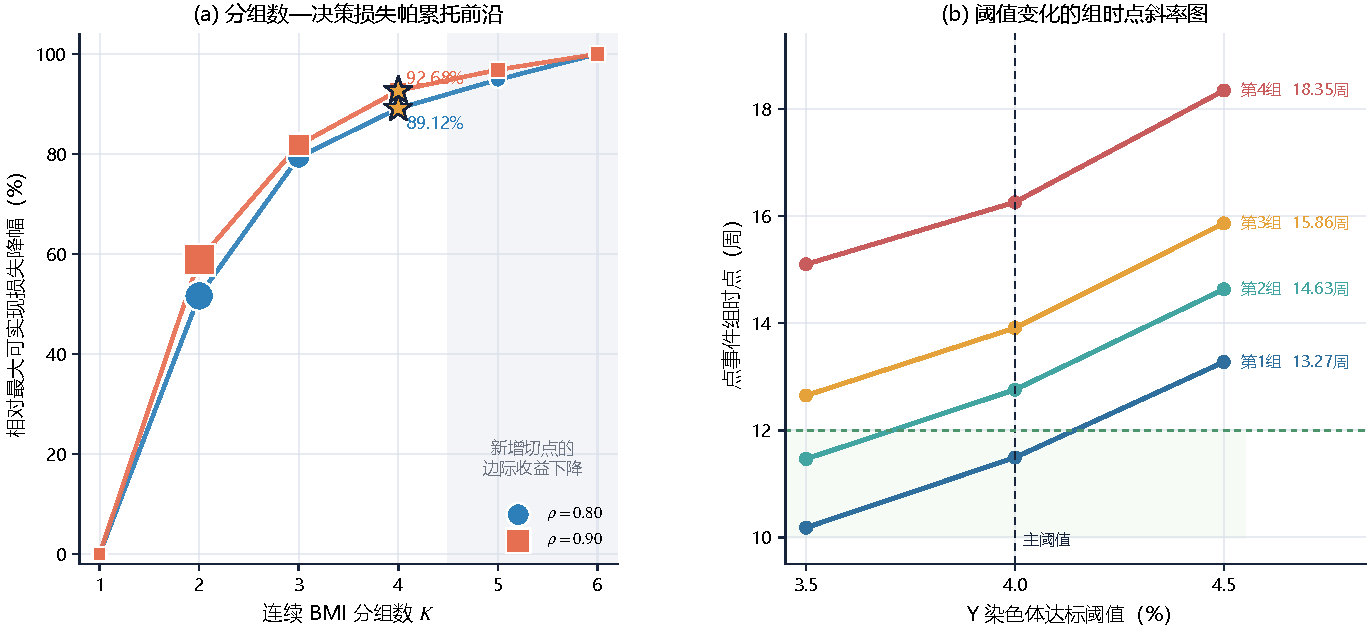
\includegraphics[width=0.98\textwidth]{figures/fig07_q2_optimization_sensitivity.pdf}
\caption{连续 BMI 分组数的决策损失帕累托前沿与 Y 染色体达标阈值的时点灵敏性}
\label{fig:q2-sensitivity}
\end{figure}

\subsection{6.11 问题二结论}\label{ux95eeux9898ux4e8cux7ed3ux8bba}

问题二的主方案取 \(\rho=0.80\)。BMI 分组为
\([20.70,31)\)、\([31,33.5)\)、\([33.5,36)\) 和
\([36,46.88]\)。推荐检测时点依次为 12 周+6 天、14 周、15 周+4 天和 19
周+6 天。四个时点均位于 25 周以内，个体保守覆盖率达到或超过 80\%。

对检测失败或漏报代价较高的情形，\(\rho=0.90\) 方案将前三组时点调整为 16
周+2 天、17 周+6 天和 20 周+2 天。BMI 不低于 36
的组在常规窗口内无法统一满足 90\%
保守覆盖，应根据已观测浓度安排复检。这一结论把高 BMI
尾部的样本稀疏和时点不确定性直接转化为可执行的检测建议。

\FloatBarrier

\section{7
问题三：多因素增量与分组修正}\label{ux95eeux9898ux4e09ux591aux56e0ux7d20ux589eux91cfux4e0eux5206ux7ec4ux4feeux6b63}

\subsection{7.1
嵌套建模思路}\label{ux5d4cux5957ux5efaux6a21ux601dux8def}

问题二已经将观测浓度转换为删失达标时间，并用 BMI
建立了四组规则。问题三保留同一采血事件定义、同一 \((L_i,R_i]\)
以及同一可靠度
\(\rho\)，将年龄、身高、孕次、产次和受孕方式作为检测前可得的增量信息。比较对象也保持不变：模型需要给真实删失区间分配较高概率，并在
12---20 周对达标概率保持较小误差。

这种嵌套关系使问题三的结论具有明确去向。若多因素改善了样本外时间预测，就用新模型重算个体保守时点，再将这些时点送入式（34）---（35）的动态规划。样本外指标变差时，问题二的
BMI 分组与时点继续作为问题三的答案。

\subsection{7.2 多因素区间删失
AFT}\label{ux591aux56e0ux7d20ux533aux95f4ux5220ux5931-aft}

对连续变量作中心化和尺度标准化，定义孕妇 \(i\) 的预测式

\[
\eta_i
=\alpha_0+\beta_BB_i^*
+\beta_AA_i^*
+\beta_HH_i^*
+\beta_GG_i^*
+\beta_PP_i^*
+\beta_CC_i,
\tag{37}
\]

其中 \(A_i\)、\(H_i\)、\(G_i\)、\(P_i\)
分别表示年龄、身高、孕次和产次，\(C_i\)
表示受孕方式的类别指示变量。对数正态 AFT 写为

\[
\log T_i=\eta_i+\sigma\varepsilon_i,
\qquad \varepsilon_i\sim N(0,1).
\tag{38}
\]

区间似然沿用式（19），并将 \(F_i(t)\) 中的 BMI 线性预测式替换为
\(\eta_i\)。为便于识别新因素的贡献，候选模型按变量块逐层扩展：

\[
\begin{aligned}
\mathcal M_0 &: BMI,\\
\mathcal M_1 &: BMI+Age+Height,\\
\mathcal M_2 &: \mathcal M_1+Gravidity+Parity+Conception.
\end{aligned}
\tag{39}
\]

BMI
由体重和身高计算而得，三者具有确定性关系。为检查体型参数化方式的影响，额外建立``体重+身高''全因素模型。该模型与
BMI 全因素模型互为替代，系数解释中不将 BMI、体重和身高作为三个独立效应。

\subsection{7.3
增量信息的评价准则}\label{ux589eux91cfux4fe1ux606fux7684ux8bc4ux4ef7ux51c6ux5219}

对每一个外层评价组，使用其余孕妇估计模型。同一孕妇的全部观测保持同组。设待评价孕妇的真实删失区间为
\((L_i,R_i]\)，模型分配给该区间的概率为

\[
\widehat q_i=
\begin{cases}
\widehat F_i(R_i), & L_i=0,\\
\widehat F_i(R_i)-\widehat F_i(L_i), & 0<L_i<R_i<+\infty,\\
1-\widehat F_i(L_i), & R_i=+\infty.
\end{cases}
\tag{40}
\]

样本外负对数似然为

\[
NLL=-\frac{1}{n_{test}}
\sum_{i\in test}
\log\{\max(\widehat q_i,\epsilon)\}.
\tag{41}
\]

NLL 越小，模型给真实达标区间分配的概率越大，其中 \(\epsilon\)
为防止概率取 0 的小正数。在 \(\mathcal T=\{12,14,16,18,20\}\)
周上还比较达标概率的 Brier 分数。对时点
\(t\)，可确定达标状态的孕妇集合为

\[
\mathcal D_t=\{i:R_i\le t\}\cup\{i:L_i\ge t\}.
\]

对 \(i\in\mathcal D_t\)，令
\(o_i(t)=\mathbf1\{R_i\le t\}\)。真实达标时间仍落在 \((L_i,R_i]\)
内的孕妇不参与该时点的 Brier 计算。多时点平均 Brier 分数写为

\[
BS=
\frac{1}{|\mathcal T|}
\sum_{t\in\mathcal T}
\frac{1}{|\mathcal D_t\cap test|}
\sum_{i\in\mathcal D_t\cap test}
\left\{\widehat F_i(t)-o_i(t)\right\}^2.
\tag{42}
\]

多因素模型相对 BMI-only 模型的改善定义为

\[
\Delta NLL=NLL_{BMI}-NLL_{multi},
\qquad
\Delta BS=BS_{BMI}-BS_{multi}.
\tag{43}
\]

正值表示多因素模型改善了样本外预测，负值表示新增变量增大了误差。每一次划分都在相同孕妇组上评价基准模型和候选模型，因此差值可在孕妇层面配对计算。

\subsection{7.4
多因素模型比较}\label{ux591aux56e0ux7d20ux6a21ux578bux6bd4ux8f83}

表~\ref{tab:q3-aft-comparison} 给出重复孕妇分组比较的平均结果。BMI-only 模型同时取得最小 NLL
和最小 Brier 分数。BMI+年龄+身高的 NLL 增加 0.01021，Brier 分数增加
0.00101。全因素模型的误差增幅更大。

\begin{table}[!htbp]
  \centering
  \caption{多因素区间删失 AFT 模型的样本外增量比较}
  \label{tab:q3-aft-comparison}
  \small
  \begin{tabularx}{\textwidth}{@{}P{3.2cm}Q{2.2cm}Q{2.7cm}Q{1.8cm}Q{1.8cm}X@{}}
    \toprule
    模型 & 样本外 NLL & 多时点平均 Brier & \(\Delta NLL\) & \(\Delta BS\) & 决策 \\
    \midrule
    BMI-only AFT & 0.690854 & 0.102167 & 基准 & 基准 & 保留 \\
    BMI+年龄+身高 & 0.701067 & 0.103177 & -0.010212 & -0.001010 & 不替换基准 \\
    BMI 全因素 & 0.785674 & 0.106613 & -0.094819 & -0.004445 & 不替换基准 \\
    体重+身高全因素 & 0.785214 & 0.106372 & -0.094359 & -0.004205 & 不替换基准 \\
    \bottomrule
  \end{tabularx}
\end{table}

BMI+年龄+身高模型的 95\% 配对区间为

\[
\Delta NLL\in[-0.029879,0.000137],
\qquad
\Delta BS\in[-0.004159,0.000667].
\]

两个区间的主要部分位于 0 以下。BMI 全因素模型的配对区间为

\[
\Delta NLL\in[-0.121279,-0.072342],
\qquad
\Delta BS\in[-0.009457,-0.001836].
\]

样本外误差增加具有一致方向。体重+身高的替代参数化得到相同结论。

加入新增变量后，小样本下的估计方差上升，不同删失类型中的局部关联稳定性下降。基线
BMI
的时间比已有明确的数据支持，年龄、身高与孕产史未在现有样本中形成可重复的增量。问题三沿用问题二的
BMI-only AFT 模型，个体时点、切点及组时点不做修改。

\subsection{7.5
达标概率与分组决策的一致性}\label{ux8fbeux6807ux6982ux7387ux4e0eux5206ux7ec4ux51b3ux7b56ux7684ux4e00ux81f4ux6027}

对给定 BMI 组 \(G_k\) 和孕周 \(t\)，平均达标概率为

\[
\bar p_k(t)
=\frac{1}{n_k}
\sum_{i\in G_k}\widehat F_i(t),
\tag{44}
\]

达到个体可靠度 \(\rho\) 的成员比例为

\[
C_k(t;\rho)
=\frac{1}{n_k}
\sum_{i\in G_k}
\mathbf1\{\widehat F_i(t)\ge\rho\}.
\tag{45}
\]

式（44）描述组平均水平，式（45）直接衡量满足个体可靠度的成员数。问题二的推荐时点使
\(C_k(t;\rho)\ge\rho\)，即组内至少有 \(\rho\)
比例成员达到个体可靠度。式（45）把成员覆盖与组平均分开。多因素 AFT
的增量比较也在这一决策尺度上完成，所以保留 BMI-only
同时意味着问题二的覆盖约束继续成立。

\subsection{7.6
随机森林的非线性增量}\label{ux968fux673aux68eeux6797ux7684ux975eux7ebfux6027ux589eux91cf}

为识别线性 AFT 可能遗漏的非线性，将每次访视在对应孕周是否达到 4\%
构造为辅助二元任务。数据划分仍以孕妇为单位，分别比较 BMI-only
和全特征逻辑回归、BMI-only 和全特征随机森林。表~\ref{tab:q3-ml-comparison}
给出四个辅助模型的评价指标。

\begin{table}[!htbp]
  \centering
  \caption{达标概率辅助模型的孕妇级样本外性能}
  \label{tab:q3-ml-comparison}
  \small
  \begin{tabularx}{0.82\textwidth}{@{}P{4.4cm}CCC@{}}
    \toprule
    辅助模型 & ROC-AUC & PR-AUC & Brier 分数 \\
    \midrule
    BMI-only 逻辑回归 & 0.81235 & 0.96706 & 0.17390 \\
    全特征逻辑回归 & 0.77384 & 0.95150 & 0.17473 \\
    BMI-only 随机森林 & 0.77534 & 0.95850 & 0.13563 \\
    全特征随机森林 & 0.81539 & 0.96839 & 0.11460 \\
    \bottomrule
  \end{tabularx}
\end{table}

全特征随机森林相对 BMI-only 森林的 ROC-AUC 增量为 0.04006，95\% 区间为
\([0.00502,0.06986]\)；Brier 分数降低 0.02103，区间为
\([0.01392,0.02788]\)。PR-AUC 增量为 0.00989，区间
\([-0.00012,0.02081]\) 跨越
0。这说明年龄、身高和孕产史中存在一定的局部非线性信息，对访视层的达标状态判别有补充作用。

问题三的决策对象是区间删失时间分布和高分位组时点。随机森林在访视层二元任务上显示了非线性信息，当前作为达标状态的辅助判别；BMI
分组与时点继续由样本外 NLL 和 Brier 分数均较低的 BMI-only AFT
给出。

图 \ref{fig:q3-increment}
将统计主线与非线性辅助线放在同一增量尺度上。左图显示 BMI-only AFT
同时位于 NLL 与 Brier 较低的区域；右图则显示多因素 AFT
的配对增量主要为负，而随机森林在 ROC-AUC 和 Brier 分数上保留正向增量。

\begin{figure}[!htbp]
\centering
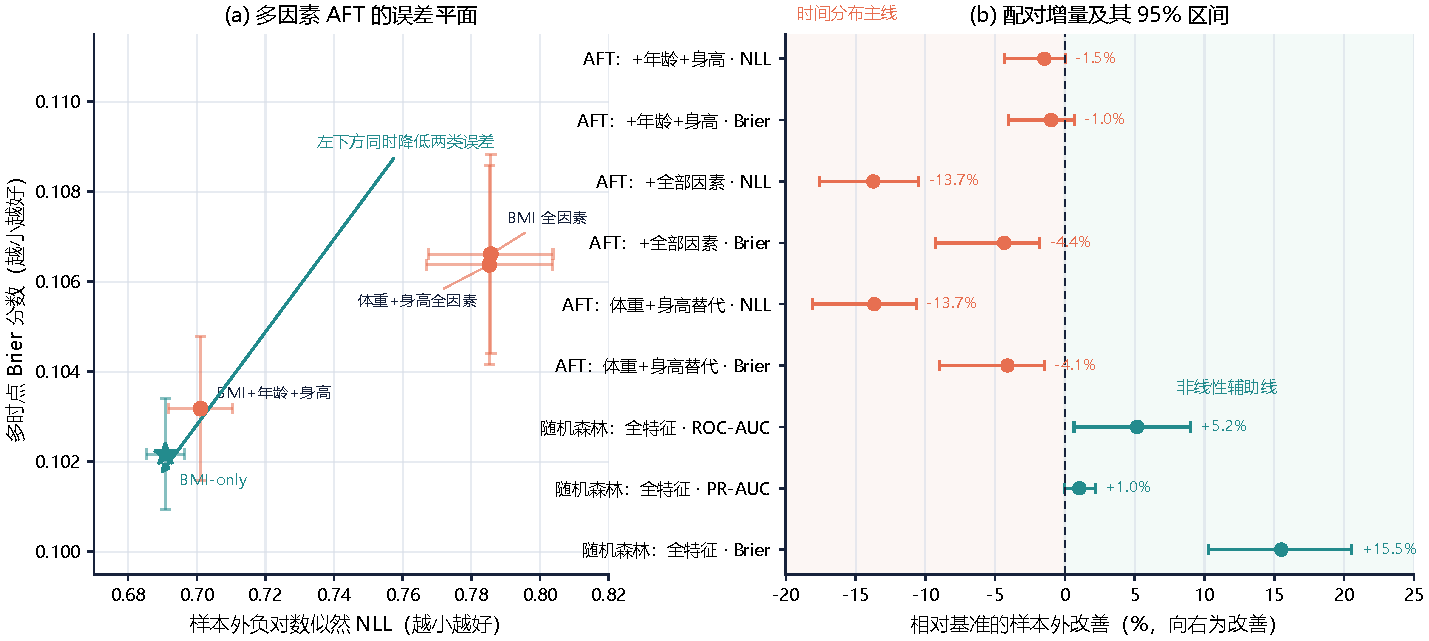
\includegraphics[width=\textwidth]{figures/fig08_q3_increment_evidence.pdf}
\caption{多因素 AFT 的样本外误差平面与统计模型、机器学习候选的配对增量区间}
\label{fig:q3-increment}
\end{figure}

\subsection{7.7
检测失败与重测延迟情景}\label{ux68c0ux6d4bux5931ux8d25ux4e0eux91cdux6d4bux5ef6ux8fdfux60c5ux666f}

附件没有独立的实验室检测失败标签，因而将失败概率作为决策参数。设首次检测失败概率为
\(\pi_f\)，失败后重测延迟 \(\Delta_f\) 周，在孕周 \(t\)
前获得可用达标结果的概率为

\[
P_{use,i}(t)
=(1-\pi_f)F_i(t)
+\pi_fF_i(t-\Delta_f).
\tag{46}
\]

式（46）将首次成功和失败后重测两条路径的达标概率加权。当
\(\pi_f=0.15\)、\(\Delta_f=2\) 周且 \(\rho=0.90\)
时，四组时点相对无失败情景约推迟 2、3、3 和 3 天。对应的七天取整时点为
15 周、16 周+5 天、18 周+2 天和 22 周+4 天。在 AFT
分位时点的情景计算中，四组仍位于 25
周内，说明中等失败概率主要造成数天的系统推迟。对问题二的个体 95\%
保守时点，高 BMI 组已超出窗口，其操作建议仍为个体化复检。

\subsection{7.8 问题三结论}\label{ux95eeux9898ux4e09ux7ed3ux8bba}

在相同的删失区间、孕妇划分和时点评价准则下，BMI-only AFT 的 NLL 为
0.69085，Brier 分数为
0.10217，均优于多因素候选模型。年龄、身高、孕次、产次与受孕方式没有改善达标时间的样本外分布预测。问题二的
BMI 切点 31、33.5、36 和两档推荐时点因此全部保留。

访视层的辅助比较中，全特征随机森林的 ROC-AUC 和 Brier
分数获得稳定改善，说明多因素中存在局部非线性信息。该信息用于达标状态的辅助识别，分组与高分位时点由区间删失
AFT 统一给出。在 15\% 失败概率与 2 周重测延迟的情景下，四组时点推迟约
2---3 天，问题二的分组结构保持稳定。

\FloatBarrier

\section{8
问题四：女胎染色体异常判定}\label{ux95eeux9898ux56dbux5973ux80ceux67d3ux8272ux4f53ux5f02ux5e38ux5224ux5b9a}

\subsection{8.1
标签定义与孕妇等权}\label{ux6807ux7b7eux5b9aux4e49ux4e0eux5b55ux5987ux7b49ux6743}

对女胎检测记录 \(r\)，将 AB 字段拆分为三个二元标签：

\[
y_{r,k}
=\mathbf1\{AB_r\text{ 中包含 }T_k\},
\qquad k\in\{13,18,21\}.
\tag{47}
\]

总体异常标签为

\[
y_{r,A}
=\max\{y_{r,13},y_{r,18},y_{r,21}\}.
\tag{48}
\]

当一条 AB 记录包含多个染色体异常时，式（47）中的多个标签可同时取
1。总体异常模型聚合了全部阳性样本，三个分型模型则分别描述染色体特征。

若孕妇 \(i\) 有 \(m_i\) 条检测记录，每条记录的基础权重设为

\[
w_{ir}=\frac{1}{m_i}.
\tag{49}
\]

因而每名孕妇的总权重均为
1。这使多次复检的孕妇与单次检测的孕妇对模型目标函数具有相同总影响。针对每个标签
\(k\)，训练数据内还按阳性与阴性的有效权重设置类别平衡因子：

\[
\widetilde w_{ir,k}
=w_{ir}
\begin{cases}
\omega_{k,+},&y_{ir,k}=1,\\
\omega_{k,-},&y_{ir,k}=0.
\end{cases}
\tag{50}
\]

记

\[
W_{k,+}=\sum_{i,r}w_{ir}\mathbf1(y_{ir,k}=1),
\qquad
W_{k,-}=\sum_{i,r}w_{ir}\mathbf1(y_{ir,k}=0).
\]

类别因子取

\[
\omega_{k,+}=\frac{W_{k,+}+W_{k,-}}{2W_{k,+}},
\qquad
\omega_{k,-}=\frac{W_{k,+}+W_{k,-}}{2W_{k,-}}.
\tag{50a}
\]

式（50a）使阳性与阴性在目标函数中的总权重相等。全部权重随后乘以同一归一化常数，类别平衡关系保持不变；式（49）的
\(1/m_i\) 因子继续限制复检次数对单名孕妇贡献的放大。

605 条女胎记录中的染色体标签可以同时出现，阳性记录不能被压缩为互斥类别：T13
与 T18 的共现记录有 11 条，T18 还分别与 T21、T13
形成小规模交集。这一结构支持 ANY 总体筛查与三个分型任务并行建模。

\subsection{8.2 特征结构}\label{ux7279ux5f81ux7ed3ux6784}

基础特征组共有 29
个原始变量，分为染色体信号、采血时点与孕妇特征、测序质量三类。染色体信号包含

\[
Z_{13},Z_{18},Z_{21},Z_X,C_X,
GC_{13},GC_{18},GC_{21},
\tag{51}
\]

其中 \(C_X\) 为 X
染色体浓度。孕妇特征包含孕周、采血次数、年龄、身高、体重、BMI、孕次、产次以及体外受精（IVF）、宫腔内人工授精（IUI）指示变量。质量变量包含总读段与唯一比对读段的对数、唯一比对比例、比对率、重复率、过滤率、总体
GC 含量以及 GC 偏离量。

对总读段数 \(N_r\) 和唯一比对读段数 \(U_r\) 作对数变换：

\[
R_r^{(N)}=\log(N_r+1),
\qquad
R_r^{(U)}=\log(U_r+1).
\tag{52}
\]

对 GC 含量构造两类绝对偏离：

\[
D_r^{GC}=|GC_r-0.5|,
\qquad
D_{r,k}^{GC}=|GC_{r,k}-GC_r|,
\quad k\in\{13,18,21\}.
\tag{53}
\]

式（52）压缩读段数的长右尾。式（53）分别刻画总体 GC 对 50\%
的偏离，以及各染色体 GC 与总体 GC 的偏离。质量信息与 Z
值共同纳入模型，使相同 Z 信号在不同读段和 GC
状态下可以得到不同风险分数。

T18 的扩展特征组在 29 个基础变量上增加 Z
值的绝对值、平方项、正负方向分段线性项以及染色体间差值和乘积，共 64
个变量。典型变换为

\[
|Z_k|,\quad Z_k^2,\quad
(Z_k-a)_+,\quad(-Z_k-a)_+,\quad a\in\{1,2,3\},
\quad Z_k-Z_{k'},\quad Z_kZ_{k'}.
\tag{54}
\]

式（54）能表示 Z
值幅度、两侧极端偏离以及染色体信号的联合结构。扩展特征还包括绝对 Z
值的最大值和平均值、三个 Z 值的标准差，以及绝对 Z 值超过 2 和 3
的染色体个数：

\[
M_Z=\max_k|Z_k|,
\quad
\overline Z_{abs}=\frac13\sum_k|Z_k|,
\quad
s_Z=\operatorname{sd}(Z_{13},Z_{18},Z_{21}),
\]

\[
N_a=\sum_{k\in\{13,18,21\}}\mathbf1\{|Z_k|\ge a\},
\qquad a\in\{2,3\}.
\]

这些变换与 29 个基础变量合计为 64
个原始特征。扩展特征在正则化下使用，参数收缩使弱信号的系数接近 0。

模型特征按题目指定的检测信息构成。AB
及其拆分标签、出生后健康结局、样本序号和孕妇编码均不作为解释变量，检测日期用于时间顺序留出验证。连续变量的缺失值取当前估计样本的中位数，并加入缺失指示变量。线性模型的中心和尺度也由当前估计样本确定，评价样本沿用对应参数。

为了在相同尺度上观察多类信号，对 29 个基础特征进行孕妇等权主成分投影。异常记录与无异常记录在前两个主成分上存在局部偏移，但各类仍大量重叠。Z
值、总体 GC 与染色体 GC
偏离的载荷方向不同，说明后续判定需要结合多类特征，不适合依赖单一 Z
值切点。

\subsection{8.3 总体异常与
T18：弹性网络逻辑回归}\label{ux603bux4f53ux5f02ux5e38ux4e0e-t18ux5f39ux6027ux7f51ux7edcux903bux8f91ux56deux5f52}

对 ANY 和 T18，使用弹性网络（Elastic Net）正则化逻辑回归。给定特征向量
\(x_r\)，异常概率为

\[
p_{r,k}
=P(y_{r,k}=1\mid x_r)
=\frac{
\exp(\beta_{0k}+x_r^{\mathsf T}\beta_k)
}{
1+\exp(\beta_{0k}+x_r^{\mathsf T}\beta_k)
}.
\tag{55}
\]

带权目标函数为

\[
\begin{aligned}
Q_k(\beta_{0k},\beta_k)
={}&-\sum_r\widetilde w_{r,k}
\left[
y_{r,k}\log p_{r,k}
+(1-y_{r,k})\log(1-p_{r,k})
\right]\\
&+\lambda_k
\left[
\alpha_k\|\beta_k\|_1
+\frac{1-\alpha_k}{2}\|\beta_k\|_2^2
\right].
\end{aligned}
\tag{56}
\]

\(L_1\) 惩罚将部分弱系数压缩为 0，\(L_2\)
惩罚稳定相关特征的系数。\(\alpha_k\) 控制两种惩罚的比例，\(\lambda_k\)
控制总收缩强度。ANY 使用 29 个基础特征，T18 使用 64
个扩展特征。两个任务的参数和阈值分别估计。

\subsection{8.4
T13：极端随机树}\label{t13ux6781ux7aefux968fux673aux6811}

T13 在 Z
值、质量偏离与孕妇特征之间呈现较强的局部交互。采用极端随机树（Extremely
Randomized Trees）构造 \(M\)
棵随机化决策树。对每个候选分裂节点，在随机选定的特征子集上生成候选分割值，再从中选择使带权类别不纯度降幅较大的分割。

第 \(m\) 棵树输出的 T13 阳性比例为 \(p_{r,13}^{(m)}\)，森林风险分数为

\[
\widehat p_{r,13}
=\frac{1}{M}
\sum_{m=1}^{M}p_{r,13}^{(m)}.
\tag{57}
\]

树的分割阈值和特征子集都具有随机性，多棵树平均可减少单树对少数阳性样本的过度依赖。模型使用
29 个基础特征，通过最小叶节样本数和最小分裂样本数控制局部分割。

\subsection{8.5
T21：收缩线性判别分析}\label{t21ux6536ux7f29ux7ebfux6027ux5224ux522bux5206ux6790}

T21 有 13 条阳性记录，对应 12 名孕妇。在 29
维特征下，普通样本协方差矩阵容易受稀少阳性的影响。收缩线性判别分析将样本协方差
\(S\) 与球形协方差组合：

\[
\widehat\Sigma_{\gamma}
=(1-\gamma)S
+\gamma\frac{\operatorname{tr}(S)}{p}I_p,
\qquad 0\le\gamma\le1.
\tag{58}
\]

设类别 \(c\in\{0,1\}\) 的均值向量和先验比例分别为 \(\mu_c\) 与
\(\pi_c\)，判别函数为

\[
\delta_c(x)
=x^{\mathsf T}\widehat\Sigma_{\gamma}^{-1}\mu_c
-\frac12\mu_c^{\mathsf T}
\widehat\Sigma_{\gamma}^{-1}\mu_c
+\log\pi_c.
\tag{59}
\]

判别顺序由 \(\delta_1(x)-\delta_0(x)\)
确定。收缩参数增大时，协方差估计更接近对角结构，可以降低高维小样本下的方差。T21
保留连续判别分数，用于辅助安排复检顺序。

\subsection{8.6
孕妇分组的嵌套评价与阈值选择}\label{ux5b55ux5987ux5206ux7ec4ux7684ux5d4cux5957ux8bc4ux4ef7ux4e0eux9608ux503cux9009ux62e9}

为使性能对应新孕妇的判定，外层按孕妇分为 4
折，并使各折阳性比例尽量接近；内层按同一原则分为 3
折。同一孕妇的所有记录在任一轮划分中始终属于同一折。整个比较使用 100
组随机划分，以分离单次划分带来的偶然波动。

对 ANY、T13 和
T18，阈值使用内层交叉验证的留出折预测选择，以下称为折外预测。定义带权混淆量

\[
TP_w=\sum_r w_r\mathbf1(y_r=1,\widehat y_r=1),
\quad
FP_w=\sum_r w_r\mathbf1(y_r=0,\widehat y_r=1),
\tag{60}
\]

\[
FN_w=\sum_r w_r\mathbf1(y_r=1,\widehat y_r=0).
\tag{61}
\]

加权精确率、召回率与 F1 值为

\[
P_w=\frac{TP_w}{TP_w+FP_w},
\qquad
R_w=\frac{TP_w}{TP_w+FN_w},
\tag{62}
\]

\[
F1_w=\frac{2P_wR_w}{P_w+R_w}.
\tag{63}
\]

对内层折外分数 \(p_r^{inner}\)，阈值为

\[
\widehat\theta_k
=\arg\max_{\theta}
F1_w\left(
\mathbf1\{p_r^{inner}\ge\theta\},y_{r,k}
\right).
\tag{64}
\]

式（64）中的每一个分数都来自未用于拟合该分数的孕妇组。外层评价时，固定模型参数和
\(\widehat\theta_k\)，再对外层留出孕妇计算式（62）---（63）与
PR-AUC、ROC-AUC。

100
组随机划分中的每一组都在本组内层预测上选择阈值。模型类型和特征组确定后，再对全部建模样本进行
5 折孕妇分组的折外预测，并按式（64）确定实际判定阈值。表~\ref{tab:q4-final-performance} 的性能是 100
组外层评价的平均值，阈值列给出最终统一判定值；两类数值分别对应泛化评价和最终规则。

除随机划分外，按孕妇的检测日期排序，使用较早 80\% 的孕妇估计模型，较晚
20\%
的孕妇评价时间顺序留出性能。这一结果衡量模型对后续检测批次和孕妇的稳定程度。

\subsection{8.7
确定模型与判定效果}\label{ux786eux5b9aux6a21ux578bux4e0eux5224ux5b9aux6548ux679c}

表~\ref{tab:q4-final-performance} 给出 100
组孕妇分组划分的平均结果。分类指标均以式（49）定义的孕妇等权为基础进行计算。加权准确率一并列出，模型取舍主要依据精确率、召回率、F1
值和 PR-AUC。

\begin{table}[!htbp]
  \centering
  \caption{女胎四项异常任务的最终模型与折外性能}
  \label{tab:q4-final-performance}
  \scriptsize
  \setlength{\tabcolsep}{1.8pt}
  \renewcommand{\arraystretch}{1.12}
  \begin{tabularx}{\textwidth}{@{}Q{0.75cm}Q{0.82cm}LQ{1.28cm}*{6}{Q{1.04cm}}@{}}
    \toprule
    任务 & \makecell{特征\\数} & 模型 & 阈值 & 精确率 & 召回率 & F1 & PR-AUC & ROC-AUC & \makecell{加权\\准确率} \\
    \midrule
    ANY & 29 & 弹性网络逻辑回归 & 0.746999 & 0.39796 & 0.48465 & 0.43203 & 0.45575 & 0.79003 & 0.85368 \\
    T13 & 29 & 极端随机树 & 0.277230 & 0.23410 & 0.44373 & 0.30165 & 0.22186 & 0.82890 & 0.91506 \\
    T18 & 64 & 弹性网络逻辑回归 & 0.744764 & 0.42366 & 0.52490 & 0.46477 & 0.47712 & 0.82473 & 0.90471 \\
    T21 & 29 & 收缩线性判别分析 & 辅助排序 & 0.04261 & 0.34619 & 0.05814 & 0.14437 & 0.46527 & 0.67784 \\
    \bottomrule
  \end{tabularx}
\end{table}

ANY 将 67 条总体阳性记录聚合为一个筛查任务，F1 值为 0.43203，PR-AUC 为
0.45575。它用于判断当前记录是否需要异常复核。T18
的阳性样本数在三个分型中最多，其精确率和召回率分别为 0.42366 和
0.52490，F1 值为四个任务中的最高值 0.46477。

T13 的精确率较低，但 ROC-AUC 达到
0.82890，说明极端随机树对风险顺序有较好区分度。阈值 0.277230 对应
0.44373 的召回率，用于触发 T13 分型复检。T21 行中的精确率、召回率和 F1
值来自候选二分规则，用于与其余任务采用同一口径比较。该任务的 ROC-AUC 为
0.46527，F1 值为 0.05814，二分结果的区分度较弱。判定方案输出 T21
连续判别分数，并按分数从高到低安排复检优先级。

图 \ref{fig:q4-score}
以折外风险分数为横轴，将真实阳性与真实阴性的加权密度分别置于基线两侧。ANY
和 T18 的阳性分布整体向高分区偏移；T13
的两类分布重叠更多，其较低阈值对应稀少阳性下的召回取舍。T21
仅保留连续排序，与其数据支持强度保持一致。

\begin{figure}[!htbp]
\centering
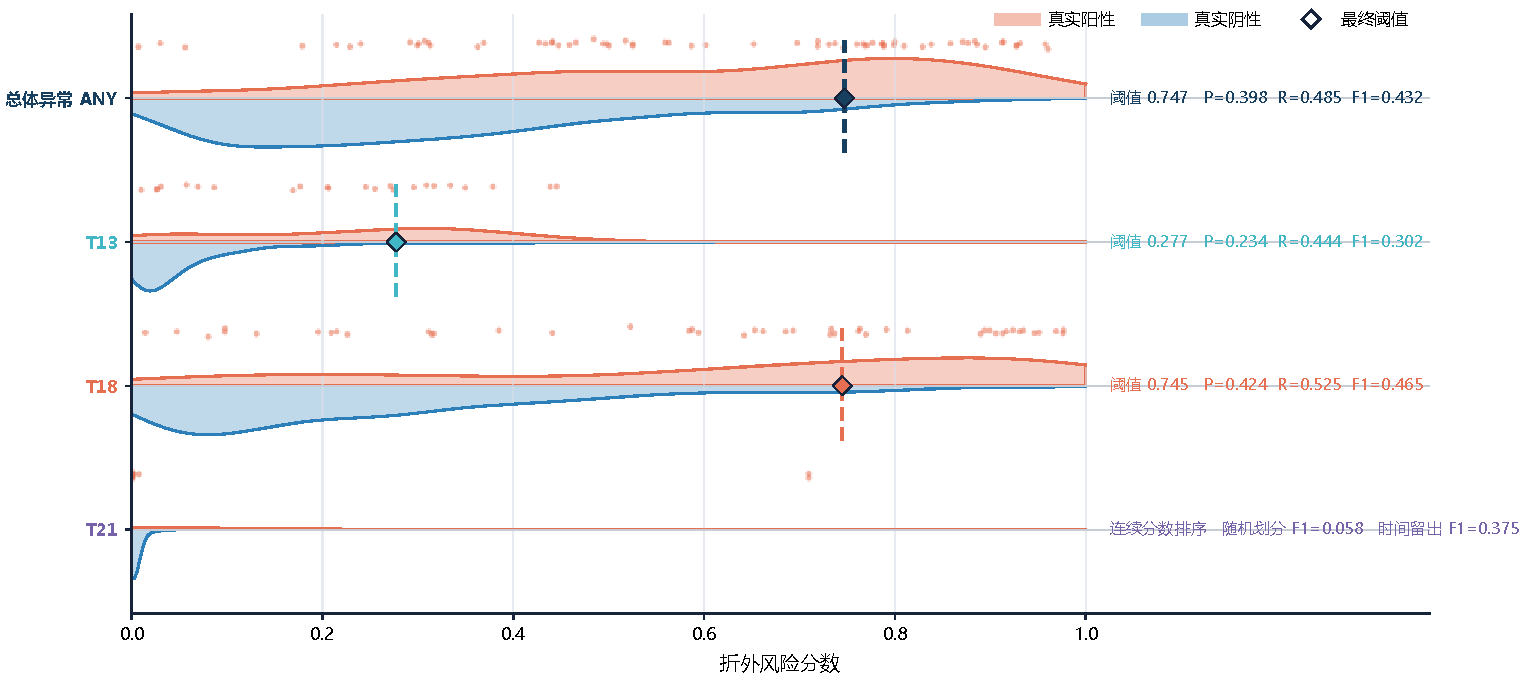
\includegraphics[width=\textwidth]{figures/fig11_q4_score_threshold_landscape.pdf}
\caption{四个女胎任务的折外风险分数镜像密度、阳性观测与最终阈值}
\label{fig:q4-score}
\end{figure}

\subsection{8.8
时间顺序留出验证与重抽样区间}\label{ux65f6ux95f4ux987aux5e8fux7559ux51faux9a8cux8bc1ux4e0eux91cdux62bdux6837ux533aux95f4}

时间顺序留出样本包含 30 名较晚检测的孕妇、共 112 条记录。ANY、T13、T18
和 T21 的带权 F1 值分别为 0.42675、0.53226、0.33437 和 0.37500。T13
在该验证中的召回率为 0.86842，PR-AUC 为
0.67137，支持保留极端随机树对局部非线性的表示。T18 的时间顺序留出 F1
值低于随机分组平均，该变化将在稳健性分析中与时间批次差异一并考察。

以所选模型的外层留出预测为基础，按孕妇整体重抽样 500
次，并在每次样本上重新计算性能。表~\ref{tab:q4-bootstrap-f1} 给出 F1 值的重抽样分布。

\begin{table}[!htbp]
  \centering
  \caption{女胎四项任务 F1 值的孕妇簇重抽样分布}
  \label{tab:q4-bootstrap-f1}
  \small
  \setlength{\tabcolsep}{4pt}
  \begin{tabularx}{\textwidth}{@{}Q{1.25cm}Q{2.0cm}Q{2.0cm}Q{3.6cm}X@{}}
    \toprule
    任务 & F1 均值 & 中位数 & 95\% 区间 & 解释 \\
    \midrule
    ANY & 0.48219 & 0.48543 & [0.35997, 0.59831] & 总体异常筛查在重抽样中保持中等识别度 \\
    T13 & 0.39300 & 0.39457 & [0.21412, 0.58532] & 阳性孕妇较少，区间较宽 \\
    T18 & 0.48974 & 0.48866 & [0.33538, 0.64228] & 三个分型中稳定性较好 \\
    T21 & 0.14190 & 0.14286 & [0.00000, 0.31684] & 下限为 0，保留连续判别分数 \\
    \bottomrule
  \end{tabularx}
\end{table}

区间宽度随阳性孕妇数减少而扩大。T18 有 30 名阳性孕妇，F1 区间下限为
0.33538；T21 有 12 名阳性孕妇，其下限降至
0。模型输出方式因而随数据支持强度变化：ANY、T13 和 T18
使用阈值触发复检，T21 保留连续判别分数。

\subsection{8.9
特征精简与方法对照}\label{ux7279ux5f81ux7cbeux7b80ux4e0eux65b9ux6cd5ux5bf9ux7167}

对 ANY，29 个基础特征的弹性网络逻辑回归相对 64 个扩展特征的候选模型，F1
平均提高 0.01584。PR-AUC 提高 0.05667，其配对 95\% 区间为
\([0.00273,0.11125]\)。时间顺序留出 F1 也由 0.40822 提高到
0.42675。这些结果支持对 ANY 使用 29 个基础特征。

对 T13，29 特征极端随机树相对 157 个纵向扩展特征的候选模型，F1 平均提高
0.02261。配对区间 \([-0.18990,0.17104]\) 较宽。时间顺序留出 F1 由
0.32500 提高到 0.53226，而特征数从 157 降至 29。T13
的极端随机树因此定位为非线性分型辅助，其阳性输出触发复检。

对 T18，29 特征模型的平均 F1 比 64 特征模型高 0.00014，但召回率从
0.52490 降至 0.49600。时间顺序留出 F1 也从 0.33437 降至 0.17082。T18
保留 64
个扩展特征和弹性网络逻辑回归。该取舍使特征精简服务于新孕妇外推，模型复杂度由样本外表现决定。

为比较复杂度与识别度，表~\ref{tab:q4-ablation}
列出最终方法、梯度提升树和基于少量质量指标的逻辑回归。三个候选均按孕妇划分数据。最终方法按
100 组随机划分计算，梯度提升树与质量指标候选分别使用 3 组和 20
组划分；最终模型的确定仍依据 100 组配对比较。

\begin{table}[!htbp]
  \centering
  \caption{女胎最终方法与简化候选模型的 F1 对照}
  \label{tab:q4-ablation}
  \small
  \begin{tabularx}{0.88\textwidth}{@{}Q{1.6cm}CCC@{}}
    \toprule
    任务 & 最终方法 F1 & 梯度提升树 F1 & 质量指标逻辑回归 F1 \\
    \midrule
    ANY & 0.43203 & 0.33879 & 0.11779 \\
    T13 & 0.30165 & 0.22280 & 0.10714 \\
    T18 & 0.46477 & 0.34191 & 0.06610 \\
    T21 & 0.05814 & 0.02037 & 0.02214 \\
    \bottomrule
  \end{tabularx}
\end{table}

梯度提升树在四个任务上的 F1
均低于最终方法。质量指标逻辑模型按高特异目标选择阈值，四个任务的特异度为
0.975 至 0.991，召回率为 0.018 至
0.075。它适合作为高特异规则的参照；平衡筛查仍需把质量信息与 Z 值、X
浓度和孕妇特征共同建模。

图 \ref{fig:q4-stability} 将各类候选模型的孕妇等权 PR-AUC 与 F1
同时展开，星标为锁定方案，误差线为 500 次孕妇簇重抽样区间。T13
的极端随机树明确高于该任务的线性候选，是机器学习对主线结论贡献较清晰的环节。时间顺序留出中
T13 的 F1 上升，T18 则表现出较高的批次敏感性。

\begin{figure}[!htbp]
\centering
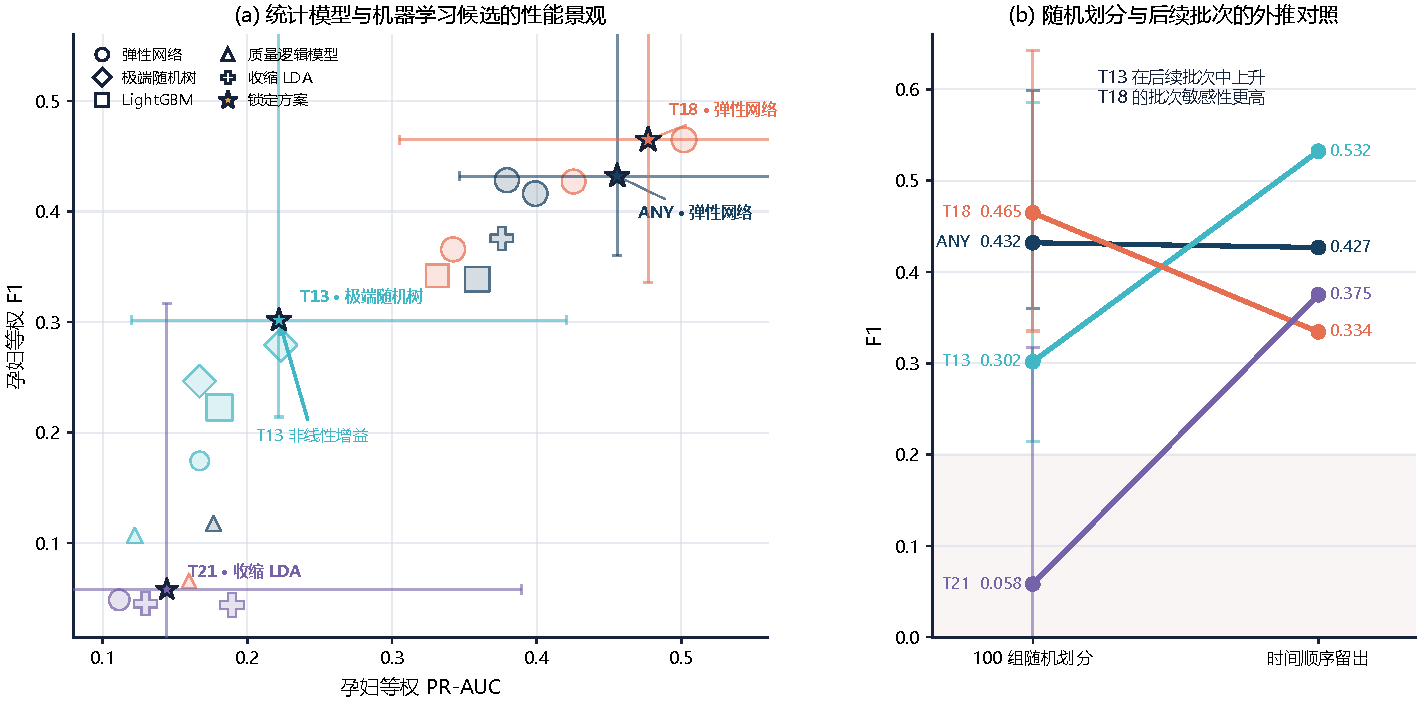
\includegraphics[width=\textwidth]{figures/fig12_q4_model_stability.pdf}
\caption{女胎候选模型的性能景观、孕妇簇 Bootstrap 区间与时间顺序留出对照}
\label{fig:q4-stability}
\end{figure}

\subsection{8.10
异常判定规则}\label{ux5f02ux5e38ux5224ux5b9aux89c4ux5219}

对每条女胎记录，计算 ANY、T13 和 T18 的风险分数。三个二元复检信号为

\[
d_{r,A}=\mathbf1(\widehat p_{r,A}\ge0.746999),
\tag{65}
\]

\[
d_{r,13}=\mathbf1(\widehat p_{r,13}\ge0.277230),
\qquad
d_{r,18}=\mathbf1(\widehat p_{r,18}\ge0.744764).
\tag{66}
\]

\(d_{r,A}=1\) 表示总体异常风险达到复核阈值，\(d_{r,13}\) 和 \(d_{r,18}\)
给出分型方向。三个信号可以同时为 1。T21 使用
\(s_{r,21}=\delta_1(x_r)-\delta_0(x_r)\)
排序，在同等复检资源下优先复核分数较高的记录。

对全部 605 条女胎记录应用式（65）---（66）后，ANY、T13 和 T18 分别有
81、43 和 51 条记录触发复检信号。T21
的全部记录保留连续排序。该操作规则将模型阳性解释为复检优先信号，后续复核可结合原始
Z 值、GC 偏离、读段质量和同一孕妇的历次记录。

\subsection{8.11 问题四结论}\label{ux95eeux9898ux56dbux7ed3ux8bba}

女胎异常判定由总体异常筛查和染色体分型组成。ANY 使用 29
特征弹性网络逻辑回归，复检阈值为 0.746999；T13 使用 29
特征极端随机树，阈值为 0.277230；T18 使用 64
特征弹性网络逻辑回归，阈值为 0.744764。三个任务的 F1 值分别为
0.43203、0.30165 和 0.46477。

T21 阳性样本量有限、区分度不足，无法设定统一二分阈值，故保留连续判别分数用于复检队列排序。T13
是第四问中机器学习增益最清晰的局部环节：极端随机树在时间顺序留出验证中的
F1 值为 0.53226，通过 29 个基础特征刻画局部非线性。ANY 与 T18
的主要信号由正则化统计模型捕捉。

\FloatBarrier

\section{9
稳健性、灵敏性与外推分析}\label{ux7a33ux5065ux6027ux7075ux654fux6027ux4e0eux5916ux63a8ux5206ux6790}

\subsection{9.1
重抽样单位与统计量}\label{ux91cdux62bdux6837ux5355ux4f4dux4e0eux7edfux8ba1ux91cf}

四个问题都包含同一孕妇的重复记录，自助法重抽样（Bootstrap）以孕妇为单位。对第
\(b\)
次抽样，有放回地选取孕妇，并保留被选孕妇的全部采血事件和技术记录。若关心的统计量为
\(\psi\)，500 次重抽样得到

\[
\widehat\psi^{(1)},\widehat\psi^{(2)},
\ldots,\widehat\psi^{(500)}.
\tag{67}
\]

其中位数用于表示稳定中心，2.5\% 和 97.5\% 分位数构成 95\%
区间。男胎流程在每次抽样中重算技术误差、达标区间、AFT 参数、个体时点和
BMI
分组，因此区间同时反映样本构成与参数估计的波动。女胎模型在随机划分下的性能波动由
100 组划分衡量；500 次 Bootstrap
以最终模型的外层留出预测为基础，用于估计性能指标随孕妇构成变化的区间。

\subsection{9.2
问题一的参数稳定性}\label{ux95eeux9898ux4e00ux7684ux53c2ux6570ux7a33ux5b9aux6027}

孕周、基线 BMI 与 18 周后的正部项在 500
次以孕妇为簇的重抽样中，系数方向保持率均为 100\%。18 周前孕周系数区间为
\([0.01294,0.03380]\)，18 周后总斜率区间为 \([0.05012,0.07514]\)。基线
BMI 系数区间为 \([-0.05727,-0.01528]\)。三个区间均与模型主结论同向。

孕期内 BMI 变化的系数区间为 \([-0.02070,0.04322]\)，正值频率为
81.6\%。该项在不同抽样中对应较大方差，而基线 BMI 的负向关系稳定。以首次
BMI 建立问题二的分组因此具有与参数稳定性相符的依据。

线性混合模型与分段线性混合模型的 RMSE
差异在所有重复划分中都很小，关系解释由似然比检验和系数区间支持。随机森林相对岭回归的
RMSE 改善在 100\%
的划分中为正，说明局部非线性预测增益不由某一次样本划分驱动。

孕周聚合序列的诊断检验包含三类统计量：达标率全局小波方差、Y 浓度 PACF 与
Lomb--Scargle 尺度谱，用于考察序列的局部结构。18
周分段模型的参数估计与后续分组规则不变。

\begin{figure}[!htbp]
  \centering
  \includegraphics[page=4,width=\textwidth]{NIPT_真实数据参考组图复现.pdf}
  \caption*{补充诊断：达标率全局小波方差、Y 浓度 PACF 与 Lomb--Scargle 尺度谱}
\end{figure}

\subsection{9.3
问题二的切点与时点稳定性}\label{ux95eeux9898ux4e8cux7684ux5207ux70b9ux4e0eux65f6ux70b9ux7a33ux5b9aux6027}

在浓度技术误差扰动的 500 次重抽样中，\(\rho=0.80\)
的三个原始切点中位数为 30.909、33.310 和 35.788；\(\rho=0.90\) 时为
30.731、33.227 和 35.614。两档可靠度的切点中心都与 31、33.5、36
的舍入规则接近。

第二、第三个原始切点在部分重抽样中出现相邻分割模式，所以切点边际区间较宽。从孕妇成员层面观察，\(\rho=0.80\)
时个体与最终分组一致的平均频率为 0.8821，中位数为 0.9300；\(\rho=0.90\)
时分别为 0.8256 和 0.8740。在两种可靠度下，分组波动主要集中在 31、33.5
和 36 附近的孕妇，距离切点较远的成员具有更高的归组频率。

固定舍入切点并重算保守时点后，\(\rho=0.80\) 四组满足覆盖约束的 Bootstrap
概率均不低于 0.952。具体数值为 0.954、0.960、0.952 和
0.952。\(\rho=0.90\) 时，对应概率为 0.958、0.964、0.950 和
0.950。切点取整后的组覆盖仍具有至少 95\% 的重抽样保证概率。

图~\ref{fig:bootstrap-decision-stability} 将不确定性沿“参数—切点—归组—排程”顺序传递。孕周效应与基线
BMI 效应的 95\% 区间保持同向，孕期内 BMI 变化的区间跨过零点。三个优化切点的分布中心接近
31、33.5 和 36，归组概率图进一步将波动定位到三个边界附近。在最终排程中，\(\rho=0.90\)
的最高 BMI 组穿过 25 周边界，正式时点为 28 周+3 天，决策由统一排程转为个体化复检。

\begin{figure}[!htbp]
  \centering
  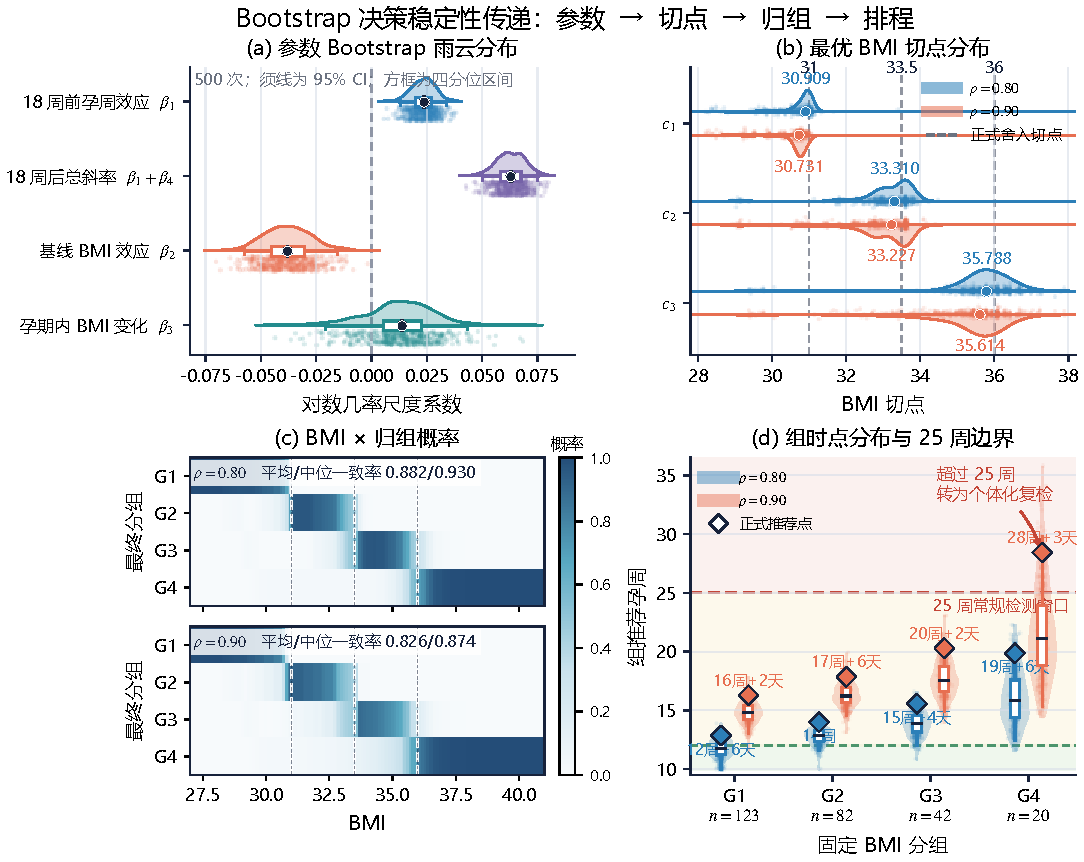
\includegraphics[width=\textwidth]{figures/fig13_bootstrap_decision_stability.pdf}
  \caption{从参数估计到分组排程的 Bootstrap 决策稳定性传递}
  \label{fig:bootstrap-decision-stability}
\end{figure}

\subsection{9.4
阈值与可靠度的灵敏性}\label{ux9608ux503cux4e0eux53efux9760ux5ea6ux7684ux7075ux654fux6027}

将 Y 浓度达标阈值从 4.0\% 分别调整为 3.5\% 和
4.5\%，在点事件误差定义下重新估计时间分布。\(\rho=0.80\)
时，三种阈值都得到约 31.03、33.62、36.10 的原始切点。表~\ref{tab:sensitivity-threshold}
列出固定点事件定义下的组时点，用于分离浓度阈值本身的影响；正式推荐还包含式（26）的技术误差保守量。

\begin{table}[!htbp]
  \centering
  \caption{Y 染色体达标阈值变化下的四组推荐时点}
  \label{tab:sensitivity-threshold}
  \small
  \begin{tabularx}{0.86\textwidth}{@{}Q{2.4cm}CCCC@{}}
    \toprule
    Y 浓度阈值 & 第 1 组 & 第 2 组 & 第 3 组 & 第 4 组 \\
    \midrule
    3.5\% & 10.18 周 & 11.46 周 & 12.65 周 & 15.10 周 \\
    4.0\% & 11.49 周 & 12.76 周 & 13.91 周 & 16.26 周 \\
    4.5\% & 13.27 周 & 14.63 周 & 15.86 周 & 18.35 周 \\
    \bottomrule
  \end{tabularx}
\end{table}

阈值改变了时点的绝对水平，四组切点和时点的递增顺序保持不变。这说明 BMI
分组主要由个体时间比和排序结构决定，阈值对检测时点的影响则以整体平移为主。

可靠度从 0.80 提高到 0.90 时，前三组的保守时点均向后移动。对应时点由 12
周+6 天、14 周、15 周+4 天变为 16 周+2 天、17 周+6 天、20 周+2
天。最高组从窗口内 19 周+6 天转为超出窗口的 28 周+3 天。可靠度是影响高
BMI 尾部决策类型的主要政策参数。

\subsection{9.5
问题三的配对稳定性}\label{ux95eeux9898ux4e09ux7684ux914dux5bf9ux7a33ux5b9aux6027}

BMI+年龄+身高模型相对 BMI-only 模型的 NLL 改善区间上限仅为 0.000137，其
97\% 的重复划分呈现 NLL 变差。对 BMI 全因素模型，NLL 与 Brier
改善区间均完全位于 0
以下。体重+身高替代参数化得到相同方向。三类候选中没有出现依赖某一 BMI
参数化的逆转，保留 BMI-only AFT 的结论在重复划分中稳定。

随机森林辅助任务的 ROC-AUC 和 Brier 改善区间均位于正值区域，PR-AUC
改善区间的下限为 -0.000118。机器学习增益因而集中于访视层状态判别，不改变
AFT 高分位时点和 BMI 动态规划。

\subsection{9.6
问题四的随机划分、时间顺序与特征稳定性}\label{ux95eeux9898ux56dbux7684ux968fux673aux5212ux5206ux65f6ux95f4ux987aux5e8fux4e0eux7279ux5f81ux7a33ux5b9aux6027}

第四问同时使用 100 组孕妇分组随机划分、500 次以孕妇为簇的 Bootstrap
重抽样和一次时间顺序留出验证。ANY 的随机划分 F1 为 0.43203，时间顺序留出
F1 为 0.42675，两者接近。T13 的时间顺序留出 F1
高于随机划分平均，其非线性识别在较晚检测样本中得到保留。T18
的时间顺序留出 F1 为 0.33437，低于随机划分平均
0.46477，该任务在新检测批次中需保留较高的复核比例。

ANY 使用 29 个基础特征后，PR-AUC 相对 64 特征候选的配对改善区间为
\([0.00273,0.11125]\)。ROC-AUC 改善区间为 \([0.01880,0.06130]\)。T13 从
157 个纵向特征精简到 29 个基础特征后，F1 差值的下限位于 0
以下，但时间顺序留出表现较好。这一结果支持将 T13
极端随机树作为分型辅助，并通过复检吸收小阳性带来的波动。

T21 的 Bootstrap F1 区间下限为 0，ROC-AUC 的重抽样均值为
0.44641，二分性能随孕妇构成变化较大。最终保留连续判别分数，并把 T21
复核与原始 Z 值共同排序。

\subsection{9.7
外推支持范围}\label{ux5916ux63a8ux652fux6301ux8303ux56f4}

男胎 BMI 的 1\% 与 99\% 分位数分别为 27.894 和 40.477。BMI
在该区间内时，模型受到较充足的样本支持。BMI 低于 27.894 或高于 40.477
时，预测位于观测边界；BMI 高于 42 的样本为 2
名，推荐应使用最高组的保守时点与个体复检。这种处理保留了模型的单调方向，避免在极少样本上进一步细分
BMI 区间。

女胎模型使用附件中的 Z 值、GC 和读段定义。对测序平台、GC
水平或读段分布发生变化的数据，需要重新估计变量的中心与尺度、正则化参数和式（64）的阈值。T13
和 T21
的阳性孕妇数较少，扩充外部阳性样本后，可依据同一孕妇分组准则重新判断分型模型和阈值。

\section{10
模型评价与适用性}\label{ux6a21ux578bux8bc4ux4ef7ux4e0eux9002ux7528ux6027}

\subsection{10.1 模型特点}\label{ux6a21ux578bux7279ux70b9}

本文在数据处理上统一以孕妇为决策单元。具体而言，采血事件层的复测用于估计技术误差，孕妇层的随机效应用于捕捉个体差异，孕妇级权重与分组则用于规范重复记录的贡献。这一处理框架在男胎和女胎分析中保持一致。

检测误差会传导至最终决策参数。技术标准差既可刻画数据波动，也会影响达标状态的判定、删失区间的估计与个体
95\% 保守时点的计算。高 BMI 组在 \(\rho=0.90\)
时由统一排程调整为个体复检。

区间删失 AFT 与动态规划直接回答了题目中的``BMI 区间''和``最佳时点''。AFT
使用所有左删失、区间删失和右删失信息，一维动态规划在连续分组中给出全局最优解。切点舍入后重新检查覆盖，使数学切分可以转化为整齐的
BMI 规则。

问题一中，随机森林浓度预测的 RMSE 较岭回归降低 4.762\%；问题三中，全特征随机森林降低了访视层 Brier
分数；问题四中，T13 极端随机树在时间顺序留出验证中的 F1
值为 0.53226。达标时间分布、BMI 分组与 ANY/T18
筛查仍采用统计模型计算。

\subsection{10.2
适用范围与结果边界}\label{ux9002ux7528ux8303ux56f4ux4e0eux7ed3ux679cux8fb9ux754c}

男胎检测时点模型适用于题目给定的 10---25 周检测窗口，并以 4\% 作为 Y
染色体浓度可靠达标标准。在 BMI 的 1\%---99\%
分位范围内，分组和时间比有较完整的样本支持。高 BMI
尾部的个体复检建议与当前样本密度一致。

女胎结果的监督目标为附件中的 AB 标记。ANY、T13 和 T18
的阳性信号用于安排复检，T21
用于排列复检优先级。该定位与现有阳性孕妇数、重抽样区间和外留区分度对应。当外部数据提供更多
T13 和 T21 阳性时，可以按同一孕妇级比较准则重新估计阈值，并重新判断 T21
是否具备二分条件。

问题一与问题二估计的是统计关系和达标时间分布。参数的解释围绕孕周、BMI 与
Y 浓度之间的条件关系，时点建议围绕题目给定的 4\%
阈值。模型在新地区或新测序平台上应先重新估计技术误差、浓度中心和质量变量分布，再使用上述达标时间与阈值选择框架。

\subsection{10.3
可进一步改进的方向}\label{ux53efux8fdbux4e00ux6b65ux6539ux8fdbux7684ux65b9ux5411}

高 BMI 区间的核心改进方向为提升样本密度与纵向访视次数。更密集的访视可收窄
\((L_i,R_i]\) 的区间宽度，补充 BMI 40
以上的孕妇样本能够缩小最高组的时点估计区间。新数据可沿用式（19）更新 AFT
分布，并通过式（34）---（35）重新计算切点。

女胎分型的改进重点是扩充独立阳性孕妇。T13
的非线性结构已经在时间顺序留出验证中呈现价值，新阳性样本可用于缩小精确率和召回率区间。T21
则需提高排序区分度，再根据新样本的 PR 曲线和复检代价设置阈值。

\section{11 结论}\label{ux7ed3ux8bba}

四个问题围绕观测数据的决策可靠性展开。针对男胎数据，建模纳入技术误差，聚焦达标时间估计与组覆盖约束；针对女胎数据，构建孕妇等权的多标签筛查框架。主要结论如下。

问题一的分段线性随机截距混合模型将 Y 染色体浓度的孕周效应分为 18
周前后两段。两段的对数几率周斜率分别为 0.02338 和 0.06315，基线 BMI
系数为 -0.03798。孕周增加会提高 Y 浓度，高基线 BMI
与较低浓度相对应。组内相关系数为
0.7305，孕妇间差异对纵向记录具有较大影响。

问题二以区间删失对数正态 AFT 估计达标时间，并将 0.00613
的技术标准差传递到个体 95\% 保守时点。每增加 1 个 BMI
单位，达标时间比的测量误差重抽样中位数为 1.03308。动态规划得到切点
31、33.5 和 36。在主方案 \(\rho=0.80\) 下，四组推荐时点为 12 周+6 天、14
周、15 周+4 天和 19 周+6 天。在 \(\rho=0.90\) 下，前三组为 16 周+2
天、17 周+6 天和 20 周+2 天；BMI 不低于 36 的组在 25
周内采用个体化复检。

问题三的 BMI-only AFT 样本外 NLL 为 0.69085，Brier 分数为
0.10217。加入年龄、身高、孕次、产次和受孕方式后，两项指标都没有改善，问题二的四组结构和推荐时点全部保留。随机森林在访视层达标判别中将
ROC-AUC 提高 0.04006，将 Brier 分数降低
0.02103，可用于识别多因素的局部非线性信号。在 15\% 检测失败概率和 2
周重测延迟下，四组点时点推迟约 2---3 天。

问题四的 ANY 总体筛查使用 29 特征弹性网络逻辑回归，阈值为
0.746999。精确率、召回率和 F1 分别为 0.39796、0.48465 和 0.43203。T13
使用 29 特征极端随机树，阈值为 0.277230，F1 为 0.30165；其时间顺序留出
F1 为 0.53226。T18 使用 64 特征弹性网络逻辑回归，阈值为
0.744764。精确率、召回率和 F1 分别为 0.42366、0.52490 和 0.46477。T21
使用收缩线性判别分析的判别分数辅助安排复检顺序。

\enlargethispage{2\baselineskip}

男胎分支的浓度关系、时间分布和 BMI
动态规划形成了``关系估计---可靠达标---分组排程''的连续链条。女胎分支使用相同的孕妇级统计口径，将质量变量、染色体信号和小阳性不确定性组合为复检决策。统计模型给出稳定主线，机器学习在浓度点预测、访视达标判别和
T13 分型三个环节提供了可量化的非线性补充。

\end{document}
